\documentclass[12pt]{iopart}

\usepackage[T1,T2A]{fontenc}%
\usepackage[english,russian]{babel}%
\usepackage{graphicx}%
\makeatletter
\@ifundefined{equation*}{}{%
  \expandafter\let\csname equation*\endcsname\@undefined
  \expandafter\let\csname endequation*\endcsname\@undefined}%
\makeatother
\usepackage{amsmath}%
\usepackage{amssymb}%
\usepackage{amsfonts}%
\usepackage{mathrsfs}%
\usepackage{bm}%
\usepackage{xcolor}%
\usepackage{textcomp}%
\usepackage{booktabs}%
\usepackage{array}%
\usepackage{newunicodechar}%
\providecommand{\tightlist}{\setlength{\itemsep}{0pt}\setlength{\parskip}{0pt}}
\providecommand{\texorpdfstring}[2]{#1}
\providecommand{\passthrough}[1]{#1}
\providecommand{\pandocbounded}[1]{#1}
\providecommand{\lt}{<}\providecommand{\gt}{>}
\newunicodechar{§}{\S}
\newunicodechar{→}{\ensuremath{\rightarrow}}
\newunicodechar{↔}{\ensuremath{\leftrightarrow}}
\newunicodechar{×}{\ensuremath{\times}}
\newunicodechar{·}{\ensuremath{\cdot}}
\newunicodechar{⊃}{\ensuremath{\supset}}
\newunicodechar{⊂}{\ensuremath{\subset}}
\newunicodechar{∘}{\ensuremath{\circ}}
\newunicodechar{°}{\ensuremath{^{\circ}}}
\newunicodechar{₀}{\textsubscript{0}}\newunicodechar{₁}{\textsubscript{1}}%
\newunicodechar{₂}{\textsubscript{2}}\newunicodechar{₃}{\textsubscript{3}}%
\newunicodechar{₄}{\textsubscript{4}}\newunicodechar{₅}{\textsubscript{5}}%
\newunicodechar{₆}{\textsubscript{6}}\newunicodechar{₇}{\textsubscript{7}}%
\newunicodechar{₈}{\textsubscript{8}}\newunicodechar{₉}{\textsubscript{9}}%
\newunicodechar{⁰}{\textsuperscript{0}}\newunicodechar{¹}{\textsuperscript{1}}%
\newunicodechar{²}{\textsuperscript{2}}\newunicodechar{³}{\textsuperscript{3}}%
\newunicodechar{⁴}{\textsuperscript{4}}\newunicodechar{⁵}{\textsuperscript{5}}%
\newunicodechar{⁶}{\textsuperscript{6}}\newunicodechar{⁷}{\textsuperscript{7}}%
\newunicodechar{⁸}{\textsuperscript{8}}\newunicodechar{⁹}{\textsuperscript{9}}%
\newunicodechar{⁻}{\textsuperscript{-}}\newunicodechar{≈}{\ensuremath{\approx}}%
\newunicodechar{≤}{\ensuremath{\le}}\newunicodechar{≥}{\ensuremath{\ge}}%
\newunicodechar{∼}{\ensuremath{\sim}}\newunicodechar{−}{\ensuremath{-}}%
\newunicodechar{–}{--}\newunicodechar{—}{---}%
\newunicodechar{∗}{\ensuremath{\ast}}\newunicodechar{∞}{\ensuremath{\infty}}%
\newunicodechar{∫}{\ensuremath{\int}}\newunicodechar{∝}{\ensuremath{\propto}}%
\newunicodechar{τ}{\ensuremath{\tau}}\newunicodechar{ν}{\ensuremath{\nu}}%
\newunicodechar{λ}{\ensuremath{\lambda}}\newunicodechar{σ}{\ensuremath{\sigma}}%
\newunicodechar{α}{\ensuremath{\alpha}}\newunicodechar{η}{\ensuremath{\eta}}%
\newunicodechar{β}{\ensuremath{\beta}}\newunicodechar{γ}{\ensuremath{\gamma}}%
\newunicodechar{ε}{\ensuremath{\epsilon}}\newunicodechar{φ}{\ensuremath{\varphi}}%
\newunicodechar{κ}{\ensuremath{\kappa}}\newunicodechar{μ}{\ensuremath{\mu}}%
\newunicodechar{θ}{\ensuremath{\theta}}\newunicodechar{ρ}{\ensuremath{\rho}}%
\newunicodechar{ω}{\ensuremath{\omega}}\newunicodechar{Γ}{\ensuremath{\Gamma}}%
\newunicodechar{Σ}{\ensuremath{\Sigma}}\newunicodechar{Δ}{\ensuremath{\Delta}}%
\newunicodechar{Θ}{\ensuremath{\Theta}}\newunicodechar{ℓ}{\ensuremath{\ell}}%
\newunicodechar{√}{\ensuremath{\surd}}\newunicodechar{∈}{\ensuremath{\in}}%
\newunicodechar{«}{\guillemotleft}
\newunicodechar{»}{\guillemotright}
\renewcommand{\thefigure}{S\arabic{figure}}%

\begin{document}

\title[Дополнительные материалы]{Supplementary Material — Ностальгический снос}

\author{Alexander Andriishin}

\address{Independent researcher; ORCID 0009-0000-4739-4017; alexander@andriishin.com}

\maketitle

\section{\texorpdfstring{S1. Доказательство Теоремы 1 (адиабатическое тождество \(B=K/2\) и его транзиентная реализуемость, OU)}{S1. Доказательство Теоремы 1 (адиабатическое тождество B=K/2 и его транзиентная реализуемость, OU)}}\label{s1.-ux434ux43eux43aux430ux437ux430ux442ux435ux43bux44cux441ux442ux432ux43e-ux442ux435ux43eux440ux435ux43cux44b-1-ux430ux434ux438ux430ux431ux430ux442ux438ux447ux435ux441ux43aux43eux435-ux442ux43eux436ux434ux435ux441ux442ux432ux43e-bk2-ux438-ux435ux433ux43e-ux442ux440ux430ux43dux437ux438ux435ux43dux442ux43dux430ux44f-ux440ux435ux430ux43bux438ux437ux443ux435ux43cux43eux441ux442ux44c-ou}



Теорема 1 main утверждает, что в адиабатическом OU-пределе кумулятивная избыточная потеря растёт как \(L_{\text{excess}}(t) = A t + (K/2)\ln(\lambda t) + C + o(1)\) с логарифмическим коэффициентом, равным \(K/2\), \textbf{на транзиентном окне концентрации} \(t \lesssim \tau_{\text{conc}}\) (длительность всплеска коллапса приора, S1.3a--c); асимптотически при \(t \gg \tau_{\text{conc}}\) установившийся коэффициент усиления \(g^\star\) насыщает накопление и логарифм переходит в постоянное плато \(\sim(K/2)\ln(1/g^\star)\) (S1.8a) --- структурная транзиентность, разбираемая в S1.4--S1.5. Вывод ведётся в линейно-гауссовом (калмановском) приближении наблюдательной модели и при явных допущениях (A1)--(A3) формулировки Теоремы 1 main; в частности шаг (S1.4) опирается на эвристическое сведение \(n_{\text{eff}} \asymp \lambda s\) к классу II (A3) \emph{на транзиентном окне}, а строгий переходный нестационарный фильтр оставлен открытым (§ 7 main). В этих рамках коэффициент \(K/2\) не зависит от \(\sigma\) и от кривизны модели. Вывод в пять шагов: (S1.1) сведение к скалярной задаче слежения по независимым координатам; (S1.2) ошибка слежения EWMA-фильтра в OU-среде, решение Риккати, установившийся \(g^\star\) и две временные шкалы (\(\tau_f^{\text{forget}}\) забывания и \(\tau_{\text{conc}}\) концентрации); (S1.3) разложение мгновенной избыточной потери до квадратичной формы по Фишеру; (S1.4) интегрирование на транзиентном окне, вывод коэффициента \(K/2\) и переход логарифма в плато при \(t \gg \tau_{\text{conc}}\); (S1.5) анализ конечно-амплитудной поправки \(g(\epsilon)\) и структурная недостижимость \(\hat B \to K/2\) как наклона; (S1.6) оптимальность флора как нижняя граница по всем архитектурам памяти (достаточность калмановского апостериора + MMSE, в линейно-гауссовом окне A1).



\subsection{S1.1 Тензоризация по независимым координатам}\label{s1.1-ux442ux435ux43dux437ux43eux440ux438ux437ux430ux446ux438ux44f-ux43fux43e-ux43dux435ux437ux430ux432ux438ux441ux438ux43cux44bux43c-ux43aux43eux43eux440ux434ux438ux43dux430ux442ux430ux43c}



По построению OU-параметризации (2.1) main приращения \(dW_{ij}\) независимы по \((i,j)\), ковариация диагональна, и процесс \(\theta(t) = (\theta_{ij}(t))\) распадается на \(K = k(k-1)\) независимых скалярных OU-процессов



\[d\theta_{ij} = -\lambda(\theta_{ij}-\theta_{ij}^*)\,dt + \sigma\,dW_{ij}, \qquad \mathbb{E}[\theta_{ij}(t)\theta_{ij}(s)] = \sigma_0^2\,e^{-\lambda|t-s|}.\]



Для идеального байесовского обучателя апостериор по \(\theta(t)\) факторизуется по координатам в ведущем порядке адиабатического предела (per-bit-uniformity, \cite{Andriishin2026b} Замечание 5, § S2); следовательно и мгновенная избыточная потеря, и её кумулятивная сумма аддитивны:



\begin{equation}L_{\text{excess}}(t) = \sum_{ij} L_{\text{excess}}^{(ij)}(t) \cdot (1 + o(1)), \tag{S1.1}\end{equation}



где \(L_{\text{excess}}^{(ij)}\) --- избыточная потеря на одной координате. Аддитивность взаимной информации и KL-дивергенции по независимым координатам --- стандартное тождество \cite{CoverThomas2006} гл. 2.5; в отличие от \(\chi^2\)-меры (мультипликативной по независимости), KL/MI аддитивны, что и обеспечивает переход к множителю \(K\) в итоговом коэффициенте (та же логика, что в \cite{Andriishin2026b} § S1.5). Достаточно доказать скалярный результат \(L_{\text{excess}}^{(ij)}(t) = a t + \tfrac12\ln(\lambda t) + c + o(1)\) и просуммировать по \(K\) координатам.



\emph{Координатно-свободный вывод коэффициента \(K/2\) (несущий аргумент).} Покомпонентная тензоризация (S1.1) удобна как иллюстрация, но \emph{значение} логарифмического коэффициента \(K/2\) от неё не зависит и не опирается на диагональность Фишера или независимость координат. Логарифмический член переходной концентрации (S1.4--S1.8 ниже) есть, в матричной форме, след произведения метрики Фишера на переходную апостериорную ковариацию: при концентрации апостериора с эффективным числом наблюдений \(n_{\text{eff}}\) переходная ковариация по \(\theta\) есть \(\Sigma_{\text{tr}} = (\mathcal I\,n_{\text{eff}})^{-1}\) (байесовская концентрация для \(K\)-мерного параметра), а мгновенный логарифмический вклад в избыточную потерю --- квадратичная форма (S1.5) со следом \[\tfrac12\,\mathrm{tr}\!\big(\mathcal I\cdot\Sigma_{\text{tr}}\big) = \tfrac12\,\mathrm{tr}\!\big(\mathcal I\,(\mathcal I\,n_{\text{eff}})^{-1}\big) = \tfrac12\,\mathrm{tr}(\mathrm{Id}_K)/n_{\text{eff}} = \frac{K}{2\,n_{\text{eff}}},\] поскольку \(\mathcal I\,(\mathcal I)^{-1} = \mathrm{Id}_K\) для \emph{любой} SPD Фишер-матрицы \(\mathcal I\) (диагональной или нет), а \(\mathrm{tr}(\mathrm{Id}_K) = K\). Информация Фишера сокращается \emph{тождественно} --- внутри следа, без обращения к покоординатному разложению, --- поэтому коэффициент \(K/2\) держится и тогда, когда softmax связывает логиты одной строки (Фишер недиагонален): он зависит лишь от размерности \(K = \dim\theta\), а не от структуры \(\mathcal I\) и не от per-bit-uniformity. Подстановка \(n_{\text{eff}} \asymp \lambda s\) (S1.4) и интегрирование \(\int (K/2)\,ds/s\) дают (S1.10) напрямую. Per-bit-uniformity остаётся нужна лишь для \emph{пола} C2 (§ S2, аддитивность вклада свежих битов), но \emph{не} для значения \(K/2\). Покоординатный вывод (S1.1)--(S1.10) ниже --- частный (диагональный) случай этого следа, приводимый для наглядности.



\subsection{S1.2 Ошибка слежения EWMA-фильтра и уравнение Риккати}\label{s1.2-ux43eux448ux438ux431ux43aux430-ux441ux43bux435ux436ux435ux43dux438ux44f-ewma-ux444ux438ux43bux44cux442ux440ux430-ux438-ux443ux440ux430ux432ux43dux435ux43dux438ux435-ux440ux438ux43aux43aux430ux442ux438}



Рассмотрим скалярную координату \(\theta(t)\) (индекс \(ij\) опускаем) со скрытой OU-динамикой \(d\theta = -\lambda\theta\,dt + \sigma\,dW\) (анкер \(\theta^* = 0\) без потери общности). Наблюдения дискретны (по одному измерению на шаг \(\Delta t = 1\), как в симуляциях). В линейно-гауссовом приближении вокруг текущей оценки наблюдение эквивалентно зашумлённому измерению \(dy_s = \theta(s)\,ds + \mathcal I_{\text{rate}}^{-1/2}\,dV_s\), где \(V_s\) --- стандартный винеровский процесс, а \(\mathcal I_{\text{rate}}\) --- \emph{скорость накопления информации Фишера} (Fisher rate) размерности {[}Fisher{]}\(\cdot\)время\(^{-1}\): количество фишеровской информации о \(\theta\), поступающее за единицу времени. При дискретизации \(\Delta t = 1\) с одним наблюдением на шаг \(\mathcal I_{\text{rate}} = \mathcal I\) численно (информация на шаг равна информации на единицу времени), и ниже пишем \(\mathcal I\) в смысле \(\mathcal I_{\text{rate}}\); в общем случае соответствие --- \(\mathcal I_{\text{rate}} = \mathcal I/\Delta t\).



Оптимальный байесовский фильтр для линейно-гауссовой системы со скрытым OU-состоянием --- стационарный фильтр Калмана--Бьюси \cite{KalmanBucy1961,AndersonMoore1979}. Стационарная апостериорная дисперсия (ошибка слежения) \(\Sigma_\infty := \lim_{t\to\infty}\mathbb{E}[(\hat\theta(t)-\theta(t))^2]\) --- положительный корень непрерывно-временного алгебраического уравнения Риккати (с Fisher-rate \(\mathcal I_{\text{rate}}\), размерности согласованы: \([\lambda\Sigma] = [\sigma^2] = [\mathcal I_{\text{rate}}\Sigma^2]\) --- дисперсия\(\cdot\)время\(^{-1}\))



\begin{equation}-2\lambda\Sigma_\infty + \sigma^2 - \mathcal I_{\text{rate}}\,\Sigma_\infty^2 = 0 \;\Longrightarrow\; \Sigma_\infty = \frac{-2\lambda + \sqrt{4\lambda^2 + 4\mathcal I_{\text{rate}}\sigma^2}}{2\mathcal I_{\text{rate}}} = \frac{\lambda}{\mathcal I_{\text{rate}}}\left(\sqrt{1 + \frac{\mathcal I_{\text{rate}}\sigma^2}{\lambda^2}} - 1\right). \tag{S1.2}\end{equation}



Фактор \(2\) в члене \(-2\lambda\Sigma_\infty\) --- стандартный для OU (генератор \(-\lambda\) действует на дисперсию с удвоением); управляющий безразмерный параметр сходимости \emph{слежения} --- это в точности \(\epsilon_{\text{track}} := \mathcal I_{\text{rate}}\sigma^2/\lambda^2\) (определение (2.2) main), то есть отношение Fisher-rate к темпу дрейфа, взвешенное амплитудой шума. Подчеркнём отличие от \(\epsilon = \sigma^2/\lambda\): \(\epsilon\) --- концентрация самого OU-латента, \(\epsilon_{\text{track}} = \mathcal I_{\text{rate}}\epsilon/\lambda\) --- концентрация \emph{оценки} латента фильтром; именно \(\epsilon_{\text{track}}\), а не \(\epsilon\), контролирует разложение ниже. В адиабатическом пределе \(\epsilon_{\text{track}} \ll 1\) разложение квадратного корня даёт



\begin{equation}\Sigma_\infty = \frac{\lambda}{\mathcal I}\cdot\frac{\mathcal I\sigma^2}{2\lambda^2}\left(1 + O\!\left(\tfrac{\mathcal I\sigma^2}{\lambda^2}\right)\right) = \frac{\sigma^2}{2\lambda}\left(1 + O(\epsilon_{\text{track}})\right) = \sigma_0^2\,(1 + O(\epsilon_{\text{track}})). \tag{S1.3}\end{equation}



Это \emph{стационарный} остаточный лаг фильтра: \(\Sigma_\infty = \sigma_0^2(1+O(\epsilon_{\text{track}})) \propto \sigma^2/\lambda \to 0\) в пределе OU-concentration. Эквивалентная \emph{шкала забывания} фильтра \(\tau_f^{\text{forget}} = 1/\sqrt{\lambda^2 + \mathcal I\sigma^2} \asymp 1/\lambda = \tau_E\) в адиабатическом пределе --- то есть оптимальный фильтр забывает на шкале дрейфа среды. \emph{(Терминологическое уточнение: ниже различаются две шкалы. Эта --- шкала забывания \(\tau_f^{\text{forget}} \asymp \tau_E\) --- задаёт глубину памяти фильтра. Отдельная шкала \(\tau_{\text{conc}}\) (время выхода на стационарный \(g^\star\), S1.3a) задаёт длительность переходного всплеска концентрации; в адиабатическом пределе они расходятся как \(\tau_{\text{conc}}/\tau_f^{\text{forget}} \asymp 1/g^\star = n_{\text{eff}}^\star \to \infty\) (а не \(\asymp 1/\epsilon_{\text{track}}\): поскольку \(g^\star = \tfrac12\epsilon_{\text{track}}\lambda\), имеем \(1/g^\star = 2/(\epsilon_{\text{track}}\lambda)\), см. ниже).)}



\emph{Установившийся коэффициент усиления и флор концентрации.} Стационарный фильтр Калмана имеет установившийся коэффициент усиления \(g^\star := \mathcal I_{\text{rate}}\Sigma_\infty/(1 + \mathcal I_{\text{rate}}\Sigma_\infty\,\Delta t)\), в адиабатическом пределе при \(\Delta t = 1\) ведущий член



\begin{equation}g^\star = \mathcal I_{\text{rate}}\,\Sigma_\infty\,(1+O(\epsilon_{\text{track}})) = \mathcal I_{\text{rate}}\cdot\frac{\sigma^2}{2\lambda}\,(1+O(\epsilon_{\text{track}})) = \tfrac12\,\epsilon_{\text{track}}\,\lambda\,(1+O(\epsilon_{\text{track}})) \;\propto\; \sigma^2, \tag{S1.3a}\end{equation}



то есть \(g^\star \to 0\) в адиабатическом пределе, \(g^\star \propto \sigma^2\) (линеен по дисперсии форсинга при фиксированных \(\lambda, \mathcal I_{\text{rate}}\)). Этот \(g^\star\) задаёт \emph{флор эффективного числа наблюдений}: установившийся фильтр взвешивает прошлое геометрически с множителем \((1-g^\star)\) за шаг, поэтому эффективное число накопленных информативных наблюдений насыщается на



\begin{equation}n_{\text{eff}}^\star = \frac{1-g^\star}{g^\star} \approx \frac{1}{g^\star} \quad (\text{точно } (1-g^\star)/g^\star,\ \text{ведущий член } 1/g^\star), \tag{S1.3b}\end{equation}



а не растёт неограниченно. Характерное время выхода на этот флор --- \emph{время концентрации}



\begin{equation}\tau_{\text{conc}} \asymp n_{\text{eff}}^\star \asymp 1/g^\star \;\propto\; 1/\sigma^2, \tag{S1.3c}\end{equation}



число шагов, за которое геометрическое окно фильтра заполняется. Принципиально: \(\tau_{\text{conc}} \asymp 1/g^\star \propto 1/\sigma^2\) --- это \emph{иная} шкала, чем шкала забывания \(\tau_f^{\text{forget}} \asymp \tau_E = 1/\lambda\); в адиабатическом пределе их отношение есть \(\tau_{\text{conc}}/\tau_E \asymp 1/g^\star = n_{\text{eff}}^\star \to \infty\) (физический \(\tau_{\text{conc}} = 1/(\lambda g^\star)\), делённый на \(\tau_E = 1/\lambda\), даёт ровно \(1/g^\star = n_{\text{eff}}^\star\) --- число эффективных наблюдений). Поскольку \(g^\star = \tfrac12\epsilon_{\text{track}}\lambda\) (S1.3a), это есть \(1/g^\star = 2/(\epsilon_{\text{track}}\lambda)\) --- содержит явный множитель \(1/\lambda\), поэтому отношение \(\tau_{\text{conc}}/\tau_E\) есть \(1/g^\star = n_{\text{eff}}^\star\), а \emph{не} \(1/\epsilon_{\text{track}}\). Именно \(\tau_{\text{conc}}\), а не \(\tau_E\), ограничивает окно логарифмического роста (S1.4), и его верхняя граница в адиабатическом времени есть \(\lambda\tau_{\text{conc}} \asymp 1/g^\star = n_{\text{eff}}^\star\).



\emph{Физическое происхождение адиабатической границы \(1/\sigma^2\).} Верхняя граница адиабатического окна \(t \ll 1/\sigma^2\) имеет прямой физический смысл: \(1/\sigma^2\) --- характерное время диффузионного ухода OU-латента на \(O(1)\). За время \(t\) накопленная дисперсия чисто диффузионной части OU-приращения есть \(\sigma^2 t\); при \(t \sim 1/\sigma^2\) она достигает \(O(1)\), латент успевает сместиться на масштаб самой переменной, и softmax-линеаризация (A1) вокруг текущей оценки теряет силу (точка линеаризации уходит из окрестности, в которой остаток EKF/Лаплас-приближения контролируем). Поэтому \(t \ll 1/\sigma^2\) --- не техническое, а физическое ограничение области применимости линейно-гауссова приближения.



\emph{Почему окно не открывается адиабатическим пределом (точная формулировка неразделимости).} Прежняя формулировка --- «\(\tau_{\text{conc}}\) и потолок \(1/\sigma^2\) оба \(\propto 1/\sigma^2\), потому не разделяются» --- \emph{физически неполна}: само совпадение степеней \(\sigma\) не влечёт неразделимости, ибо две величины, обе \(\propto 1/\sigma^2\), могут иметь любое постоянное отношение. Корректный аргумент --- через \emph{ширину лог-окна} и её \(\sigma\)-инвариантность. Доступное лог-несущее окно есть \([t_{\min}, t_{\max}]\) с нижней границей \(t_{\min} \asymp\) несколько \(\tau_{\text{conc}} \asymp 1/g^\star\) (логарифм жив лишь после выхода всплеска концентрации) и верхней \(t_{\max} \asymp c_0/\sigma^2\) (адиабатический потолок). Его \emph{логарифмическая ширина} (отношение границ) \[W = \frac{t_{\max}}{t_{\min}} \asymp \frac{c_0/\sigma^2}{1/g^\star} = c_0\,\frac{g^\star}{\sigma^2} \asymp \frac{\mathcal I_{\text{rate}}}{\lambda} = \frac{1}{\lambda r}\] (подставлено \(g^\star = \tfrac12\mathcal I_{\text{rate}}\sigma^2/\lambda\) из (S1.3a), \(\sigma^2\) \emph{сокращается}; \(r = 1/\mathcal I_{\text{rate}}\) --- шум наблюдения). Решающее: \textbf{ширина окна \(W \asymp 1/(\lambda r)\) \(\sigma\)-инвариантна} --- \(\sigma\) из неё ушла. Поэтому адиабатический предел \(\sigma \to 0\) (\(\epsilon_{\text{track}} \to 0\)) \emph{не открывает} лог-окно: и нижняя граница \(\tau_{\text{conc}} \propto 1/\sigma^2\), и верхняя \(1/\sigma^2\) растягиваются \emph{в одинаковой пропорции}, отношение остаётся фиксированным \(\asymp 1/(\lambda r)\). Это и есть подлинная причина неразделимости, и она \emph{рефутирует} рабочую гипотезу («толкнуть \(\epsilon_{\text{track}} \to 0\) --- окно раскроется»): уменьшение \(\sigma\) не трогает \(W\). Расширить \(W\) можно лишь увеличив Fisher-rate на корреляционный интервал среды, \(\mathcal I_{\text{rate}}/\lambda = 1/(\lambda r) \to \infty\) (бесконечно точное наблюдение \(r \to 0\) либо \(\lambda \to 0\) быстрее \(\mathcal I_{\text{rate}}\)). Но это \emph{выводит из медленно-дрейфового (адиабатического) режима}: \(\mathcal I_{\text{rate}}/\lambda \to \infty\) означает \(\epsilon_{\text{track}} = \mathcal I_{\text{rate}}\sigma^2/\lambda^2 = (\mathcal I_{\text{rate}}/\lambda)(\sigma^2/\lambda)\) перестаёт быть малым при фиксированной концентрации латента, нарушая условие slow-driving \(\lambda\tau_{\text{relax}}\ll1\) и квазистационарность \(\theta\), на которых стоят (A1) и весь вывод. Итог: неразделимость лог-несущего и асимптотического окон --- \emph{следствие адиабатического ограничения} (фиксированной Fisher-rate на корреляционный интервал), а не арифметического совпадения степеней \(\sigma\); в любом режиме, где (A1) и квазистационарность верны, \(W \asymp 1/(\lambda r) = O(1)\) относительно \(\sigma\), и лог-окно не раскрывается. Это ключ к структурной недостижимости S1.5.



Помимо стационарной части, фильтр имеет \emph{переходную} компоненту: при старте из априорной неопределённости апостериорная дисперсия \(\Sigma(t)\) убывает к \(\Sigma_\infty\). Для медленного дрейфа релевантная переходная дисперсия контролируется накоплением \emph{информативных} наблюдений. \textbf{В транзиентном режиме концентрации} (\(s \lesssim \tau_{\text{conc}}\), до выхода на установившийся \(g^\star\)) наблюдения, разнесённые более чем на \(\tau_E\), декоррелируют (ковариация \(\theta\) затухает как \(e^{-\lambda|t-s|}\)), и эффективное число независимых наблюдений о текущем \(\theta(t)\) растёт как



\begin{equation}n_{\text{eff}}(s) \asymp \frac{s}{\tau_E} = \lambda s \qquad (\text{транзиентно, } s \lesssim \tau_{\text{conc}}). \tag{S1.4}\end{equation}



Это \emph{транзиентный} (всплесковый) режим: рост (S1.4) не продолжается до \(t\to\infty\) --- при \(s \gtrsim \tau_{\text{conc}}\) установившийся \(g^\star\) (S1.3a) обрезает накопление, и \(n_{\text{eff}}\) насыщается на флоре \(n_{\text{eff}}^\star = (1-g^\star)/g^\star \approx 1/g^\star\) (S1.3b). Линейный рост \(\lambda s\) и насыщение на \(1/g^\star\) совпадают при \(s \asymp \tau_{\text{conc}}\), что и фиксирует момент перехода. \emph{Уточнение единиц времени (во избежание кажущегося двойного определения).} Время концентрации естественно записывается в двух согласованных нормировках: (a) в \emph{физическом} времени (число шагов \(s\), \(\Delta t = 1\)) переход \(n_{\text{eff}}(s) = \lambda s = n_{\text{eff}}^\star = 1/g^\star\) даёт \(\tau_{\text{conc}}^{\text{физ}} \asymp 1/(\lambda g^\star)\) --- именно эта величина измеряется числом шагов до выхода фильтра на плато; (b) в \emph{адиабатическом} времени \(u = \lambda s\) (число корреляционных интервалов среды) тот же переход есть \(u_{\text{conc}} = \lambda\,\tau_{\text{conc}}^{\text{физ}} \asymp 1/g^\star\) --- это форма (S1.3c), записанная в безразмерном \(u\) (равно \(n_{\text{eff}}^\star\), числу эффективных наблюдений). Связь: \(\tau_{\text{conc}}^{\text{физ}} = u_{\text{conc}}/\lambda\), и обе \(\propto 1/\sigma^2\) (поскольку \(g^\star \propto \sigma^2\)). Ниже под \(\tau_{\text{conc}}\) без пометки понимается физическая шкала \(1/(\lambda g^\star)\), кроме (S1.3c), где она берётся в адиабатическом \(u\). Принципиально: неразделимость \(\tau_{\text{conc}}\) и адиабатического потолка \(1/\sigma^2\) (ключ S1.5) держится в \emph{согласованной} нормировке --- в физическом времени обе \(\asymp 1/\sigma^2\), в адиабатическом обе \(\asymp \lambda/\sigma^2\); отношение, на котором стоит структурная недостижимость, нормировкой не меняется. В транзиентном окне апостериорная дисперсия по «текущему уровню» латента убывает как \(\Sigma_{\text{tr}}(s) \asymp 1/(\mathcal I\,n_{\text{eff}}(s)) = 1/(\mathcal I\lambda s)\) --- стандартная байесовская концентрация \(1/(\mathcal I n)\) с эффективным \(n = \lambda s\) \cite{ClarkeBarron1990}; асимптотически \(\Sigma_{\text{tr}} \to 1/(\mathcal I n_{\text{eff}}^\star) = \Sigma_\infty\) (флор сливается со стационарным лагом).



\subsection{S1.3 Квадратичное разложение мгновенной избыточной потери}\label{s1.3-ux43aux432ux430ux434ux440ux430ux442ux438ux447ux43dux43eux435-ux440ux430ux437ux43bux43eux436ux435ux43dux438ux435-ux43cux433ux43dux43eux432ux435ux43dux43dux43eux439-ux438ux437ux431ux44bux442ux43eux447ux43dux43eux439-ux43fux43eux442ux435ux440ux438}



Мгновенный прирост избыточной потери на шаге \(s\) --- лог-отношение правдоподобий оракула и обучателя:



\[\Delta L_{\text{excess}}(s) = \ln\frac{p(X_s\mid\theta(s))}{\hat p(X_s\mid\hat\theta(s))}.\]



Усреднение по \(X_s \sim p(\cdot\mid\theta(s))\) даёт KL-дивергенцию \(D_{KL}(p(\cdot\mid\theta(s)) \,\|\, \hat p(\cdot\mid\hat\theta(s)))\). Для регулярной параметрической модели при малой ошибке слежения \(\delta\theta := \hat\theta(s)-\theta(s)\) разложение Тейлора KL до второго порядка (первый порядок обнуляется в точке \(\theta(s)\)):



\begin{equation}\mathbb{E}[\Delta L_{\text{excess}}(s)] = \tfrac12\,\mathcal I(\theta(s))\,\mathbb{E}[\delta\theta^2] + O(\mathbb{E}|\delta\theta|^3) \tag{S1.5}\end{equation}



--- стандартное квадратичное разложение регрета по метрике Фишера \cite{ClarkeBarron1990,Rissanen1986,CoverThomas2006} гл. 11. Ошибка слежения \(\mathbb{E}[\delta\theta^2]\) распадается на стационарную и переходную части (S1.2 и S1.4):



\begin{equation}\mathbb{E}[\delta\theta^2(s)] = \underbrace{\Sigma_\infty}_{\text{стационарная}} + \underbrace{\Sigma_{\text{tr}}(s)}_{\text{переходная}} = \sigma_0^2(1+O(\epsilon_{\text{track}})) + \frac{1}{\mathcal I\lambda s}(1+o(1)). \tag{S1.6}\end{equation}



\subsection{\texorpdfstring{S1.4 Интегрирование и вывод коэффициента \(K/2\)}{S1.4 Интегрирование и вывод коэффициента K/2}}\label{s1.4-ux438ux43dux442ux435ux433ux440ux438ux440ux43eux432ux430ux43dux438ux435-ux438-ux432ux44bux432ux43eux434-ux43aux43eux44dux444ux444ux438ux446ux438ux435ux43dux442ux430-k2}



Подставляя (S1.6) в (S1.5) и интегрируя по \(s\) от некоторого \(s_0\) (после начального переходника) \textbf{на транзиентном окне концентрации \(s_0 \le s \lesssim \tau_{\text{conc}}\)}, где переходная дисперсия ещё убывает по (S1.4):



\begin{equation}L_{\text{excess}}^{(ij)}(t) = \int_{s_0}^t \tfrac12\mathcal I\left[\Sigma_\infty + \Sigma_{\text{tr}}(s)\right]ds + \text{const} = \underbrace{\tfrac12\mathcal I\Sigma_\infty\,(t-s_0)}_{\text{линейный } a\,t} + \underbrace{\frac12\int_{s_0}^{\min(t,\,\tau_{\text{conc}})}\frac{ds}{s}}_{\text{логарифмический член (S1.8)}}. \tag{S1.7}\end{equation}



Верхний предел логарифмического интеграла --- \textbf{\(\min(t,\tau_{\text{conc}})\), а не \(t\)}: подынтегральное \(\Sigma_{\text{tr}}(s) \asymp 1/(\mathcal I\lambda s)\) справедливо лишь пока \(n_{\text{eff}}(s)\asymp\lambda s\) растёт (S1.4), то есть на транзиентном окне \(s \lesssim \tau_{\text{conc}}\). При \(s \gtrsim \tau_{\text{conc}}\) установившийся \(g^\star\) насыщает \(n_{\text{eff}}\) на флоре \(1/g^\star\), переходная дисперсия выходит на \(\Sigma_\infty\), и подынтегральное \(\Sigma_{\text{tr}}\) перестаёт давать \(1/s\)-вклад --- оно поглощается стационарным членом \(\Sigma_\infty\). Это и есть структурная причина транзиентности логарифма, встроенная в механизм, а не внешняя оговорка.



Точнее: переходный вклад в (S1.5) есть \(\tfrac12\mathcal I\cdot\Sigma_{\text{tr}}(s) = \tfrac12\mathcal I\cdot\frac{1}{\mathcal I\lambda s} = \frac{1}{2\lambda s}\) за единицу \emph{физического} времени (на транзиентном окне). Сведение к \emph{адиабатическому} времени \(u = \lambda s\) (число корреляционных интервалов) --- содержательный шаг, опирающийся на допущение (A3) о концентрации класса II: переход к \(n_{\text{eff}} \asymp \lambda s\) \emph{мотивирован эвристически} аналогией с эффективным размером выборки Бартлетта \(n_{\text{eff}} = n/(1+2\sum_s\rho(s))\) \cite{Bartlett1946} для наблюдений с экспоненциальной автокорреляцией \(\rho(s) = e^{-\lambda|s|}\). \emph{Аккуратно о факторе \(\tfrac12\):} для \(\rho(s) = e^{-\lambda|s|}\) сумма автокорреляций \(1 + 2\sum_{s\ge1}\rho(s) \approx 2\sum_{s\ge0}e^{-\lambda s} \approx 2/\lambda\) при \(\lambda \ll 1\), откуда \(n_{\text{eff}} = n/(1+2\sum_s\rho) \approx n/(2/\lambda) = (\lambda/2)\,n\) --- то есть с фактором \(\tfrac12\), \(n_{\text{eff}} \approx (\lambda/2)\,n\), а \emph{не} \(\lambda n\). Этот фактор \(\tfrac12\) не исчезает бесследно: он входит лишь в \emph{аддитивную логарифмическую константу}, не в наклон, поскольку \(\ln\big((\lambda/2)s\big) = \ln(\lambda s) - \ln 2\) --- сдвиг \(-\ln 2\) на координату поглощается константой \(c_{ij}\) (и далее \(C\)) формулы (S1.9)--(S1.10), а коэффициент при \(\ln(\lambda s)\) остаётся \(\tfrac12\). Поэтому записываем \(n_{\text{eff}} \asymp \lambda n\) \emph{как порядково-точное соотношение с точностью до мультипликативной константы} \(O(1)\) (здесь \(\tfrac12\)), фиксирующее лишь \emph{показатель} \(\lambda s\) и потому наклон \(K/2\); точное значение константы влияет только на \(C\). Эта аналогия установлена Бартлеттом для оценки \emph{среднего} стационарного коррелированного процесса; её формальный перенос на \emph{слежение} за дрейфующим латентом строго не обоснован и вынесен в открытые вопросы (§ 7 main). Это \emph{эвристическое сведение к классу II} \cite{BialekNemenmanTishby2001}, а не независимый вывод; строгий контроль переходного нестационарного фильтра (нестационарное уравнение Риккати) вынесен в открытые вопросы § 7 main. Сам коэффициент ½-на-параметр --- стандартная асимптотика байесовского / MDL универсального кодирования \cite{ClarkeBarron1990,Rissanen1986,Schwarz1978}, а его сдвинутая масштабом дрейфа predictive-information-форма --- класс II \cite{BialekNemenmanTishby2001}. С этой оговоркой плотность накопления избыточной потери на единицу \(u\) есть \(\tfrac12\) (по одной координате). Эквивалентно, в физическом времени, \textbf{на транзиентном окне} \([s_0,\,\min(t,\tau_{\text{conc}})]\):



\begin{equation}\int_{s_0}^{\min(t,\,\tau_{\text{conc}})} \frac{1}{2\lambda s}\,\lambda\,ds = \frac12\int_{s_0}^{\min(t,\,\tau_{\text{conc}})}\frac{ds}{s} = \frac12\ln\frac{\min(t,\tau_{\text{conc}})}{s_0}. \tag{S1.8}\end{equation}



\textbf{Два режима по соотношению \(t\) и \(\tau_{\text{conc}}\).} (i) \emph{В транзиентном окне} \(s_0 \ll t \lesssim \tau_{\text{conc}}\) интеграл даёт \(\tfrac12\ln(t/s_0) = \tfrac12\ln(\lambda t) - \tfrac12\ln(\lambda s_0)\) --- логарифмический рост с коэффициентом \(\tfrac12\) на координату, ровно класс II \cite{BialekNemenmanTishby2001}. \emph{Именно этот режим} фиксирует аналитическое тождество \(B = K/2\) (предел \(\epsilon_{\text{track}}\to 0\)). (ii) \emph{Асимптотически} при \(t \gg \tau_{\text{conc}}\) (установившийся дрейф) интеграл обрезается сверху на \(\tau_{\text{conc}}\) и логарифмический член \emph{переходит в постоянное плато}



\begin{equation}\frac12\ln\frac{\tau_{\text{conc}}}{s_0} \asymp \frac12\ln(1/g^\star) \qquad (t \gg \tau_{\text{conc}}), \tag{S1.8a}\end{equation}



то есть на координату --- константа \(\tfrac12\ln(1/g^\star)\), суммарно по \(K\) координатам плато высотой \(\sim (K/2)\ln(1/g^\star)\). Это устраняет кажущееся противоречие между \(n_{\text{eff}}\asymp\lambda t\to\infty\) (S1.4) и насыщением \(n_{\text{eff}}\) флором: первое --- \emph{транзиентный} всплеск концентрации (\(s \lesssim \tau_{\text{conc}}\)), второе --- \emph{асимптотика} установившегося дрейфа (\(s \gtrsim \tau_{\text{conc}}\)); они относятся к разным окнам одного интеграла, а не к двум несовместимым посылкам.



Ключевой момент --- \emph{сокращение информации Фишера}: переходная дисперсия \(\Sigma_{\text{tr}}(s) = 1/(\mathcal I\lambda s)\) содержит \(1/\mathcal I\), а квадратичный множитель (S1.5) содержит \(\mathcal I\); их произведение \(\tfrac12\mathcal I\cdot 1/(\mathcal I\lambda s) = 1/(2\lambda s)\) не зависит от \(\mathcal I\). Поэтому логарифмический коэффициент определяется \emph{только размерностью}, а не кривизной модели --- это и есть универсальность класса II \cite{BialekNemenmanTishby2001}. Собирая (S1.7)--(S1.8) для одной координаты \emph{в транзиентном окне} \(s_0 \ll t \lesssim \tau_{\text{conc}}\):



\begin{equation}L_{\text{excess}}^{(ij)}(t) = a_{ij}\,t + \tfrac12\ln(\lambda t) + c_{ij} + o(1), \qquad a_{ij} = \tfrac12\mathcal I_{ij}\Sigma_\infty^{(ij)} = \tfrac12\mathcal I_{ij}\sigma_0^2(1+O(\epsilon_{\text{track}})). \tag{S1.9}\end{equation}



Суммируя по \(K\) координатам через (S1.1):



\begin{equation}L_{\text{excess}}(t) = \underbrace{\Big(\sum_{ij}a_{ij}\Big)}_{=:A}\,t + \frac{K}{2}\ln(\lambda t) + C + o(1). \tag{S1.10}\end{equation}



Логарифмический коэффициент равен \(\sum_{ij}\tfrac12 = K/2\) --- тождественно, независимо от \(\sigma\) и от значений \(\mathcal I_{ij}\). Линейный коэффициент \(A = \sum_{ij}\tfrac12\mathcal I_{ij}\sigma_0^2(1+O(\epsilon_{\text{track}})) = \tfrac12\sigma_0^2\,\mathrm{tr}\,\mathcal I\cdot(1+O(\epsilon_{\text{track}})) \propto \sigma_0^2 = \sigma^2/(2\lambda) \to 0\) при \(\epsilon \to 0\). Это доказывает транзиентную форму (3.1) main (на окне \(1\ll\lambda t\lesssim\lambda\tau_{\text{conc}}\asymp 1/g^\star\)); асимптотическую форму (3.1\('\)) main --- линию-плюс-плато \(L_{\text{excess}}(t) = At + (K/2)\ln(1/g^\star) + o(t)\) при \(t\gg\tau_{\text{conc}}\) --- даёт обрезка логарифмического интеграла на \(\tau_{\text{conc}}\) согласно (S1.8a). Обе формы --- равноправные части Теоремы 1, не «асимптотика и следствие». \(\square\)



\emph{Следствие (3.2) main.} На транзиентном окне \(1\ll\lambda t\lesssim\lambda\tau_{\text{conc}}\) (логарифмический интеграл (S1.8) обрезан сверху на \(\min(t,\tau_{\text{conc}})\) согласно (S1.8a); при \(t\gg\tau_{\text{conc}}\) член \((K/2)\ln(\lambda t)\) переходит в плато \((K/2)\ln(1/g^\star)\) и формула (3.2) перестаёт действовать) при линейном росте бюджета \(N_{\text{max}}(t) \sim Rt\) и \(L_{\text{excess}}(t) \sim (K/2)\ln(\lambda t)\) (ведущий член при \(A \to 0\)):



\[\eta_L^{\text{excess}}(t) = \frac{L_{\text{excess}}(t)}{N_{\text{max}}(t)} \sim \frac{(K/2)\ln(\lambda t)}{Rt}, \qquad \dot\eta_L^{\text{excess}}(t) = \frac{d}{dt}\frac{(K/2)\ln(\lambda t)}{Rt} = \frac{(K/2)}{Rt^2} - \frac{(K/2)\ln(\lambda t)}{Rt^2} \sim -\frac{K\ln(\lambda t)}{2Rt^2},\]



где в ведущем порядке \(\ln(\lambda t) \gg 1\) доминирует второй член. Это (3.2) main. \(\square\)



\subsection{\texorpdfstring{S1.5 Конечно-амплитудная поправка и сходимость \(\hat B \to K/2\)}{S1.5 Конечно-амплитудная поправка и сходимость \textbackslash hat B \textbackslash to K/2}}\label{s1.5-ux43aux43eux43dux435ux447ux43dux43e-ux430ux43cux43fux43bux438ux442ux443ux434ux43dux430ux44f-ux43fux43eux43fux440ux430ux432ux43aux430-ux438-ux441ux445ux43eux434ux438ux43cux43eux441ux442ux44c-hat-b-to-k2}



Истинный логарифмический коэффициент равен \(K/2\) (S1.10). Скан § S8.3 \cite{Andriishin2026b} наблюдал \(\hat B/(K/2) = 0{,}54,\ 0{,}78,\ 0{,}85\) при \(\epsilon = 10^{-1},\ 9\cdot10^{-3},\ 10^{-3}\) --- недобор, монотонно убывающий с \(\epsilon\). Покажем, что это смещение \emph{оценки} на конечном окне фита, а не свойство истинного коэффициента.



Совместная подгонка \(L_{\text{excess}}(t) \approx \hat A t + \hat B\ln(\lambda t) + \hat C\) на окне \([t_{\min}, t_{\max}]\) методом наименьших квадратов оценивает \(\hat B\) через проекцию данных на регрессор \(\ln(\lambda t)\), ортогонализованный к \(\{t, 1\}\). При конечном \(\epsilon\) линейный член \(A t\) с \(A \propto \epsilon\) велик (доля дрейфа в скане: 76\% при \(\epsilon = 10^{-1}\)), и регрессоры \(t\) и \(\ln(\lambda t)\) на конечном окне \([t_{\min}, t_{\max}]\) статистически коррелированы (оба монотонно растут). Неполная ортогонализация переносит часть дисперсии логарифмического сигнала в линейный регрессор, занижая \(\hat B\). Стандартный анализ смещения МНК при коррелированных регрессорах даёт



\begin{equation}\hat B = \frac{K}{2}\big(1 - g(\epsilon, W)\big), \qquad g(\epsilon, W) = \frac{A\cdot\mathrm{Cov}_W(t,\ \ell)}{(K/2)\cdot\mathrm{Var}_W(\ell)}\bigg|_{\ell = \ln(\lambda t)} = O\big(\epsilon\cdot\Theta(W)\big), \tag{S1.11}\end{equation}



где \(W = t_{\max}/t_{\min}\) --- отношение границ окна, \(\Theta(W)\) --- фактор перекрытия регрессоров (растёт с шириной окна), \(A \propto \epsilon\). Поскольку \(g \propto A \propto \epsilon\), имеем \(g(\epsilon) \to 0\) при \(\epsilon \to 0\), и \(\hat B \to K/2\). Качественно: \(\hat B/(K/2)\) монотонно растёт с убыванием \(\epsilon\) --- \(0{,}54 \to 0{,}78 \to 0{,}85\) при \(\epsilon: 10^{-1} \to 9\cdot10^{-3} \to 10^{-3}\) (то есть \(g(\epsilon) = 0{,}46,\ 0{,}22,\ 0{,}15\) убывает к нулю) --- что и предсказывает \(g(\epsilon) \to 0\). \emph{Точная функциональная форма \(g(\epsilon)\) оставлена открытой.} Теоретическая зависимость из (S1.11) --- линейная, \(g \propto \epsilon^1\) (через \(A \propto \epsilon\)); численная же подгонка \(g \approx 1{,}5\,\epsilon^{0{,}25}\) по трём точкам даёт показатель \(\approx 0{,}25\), не согласующийся с теоретическим \(1\). Этот показатель \emph{не выведен} и приводится лишь как грубая интерполяция по трём точкам \emph{субоптимального} Robbins--Monro-скана § S8.3 \cite{Andriishin2026b} (того самого обучателя, дезавуированного ниже как «отрицательный контроль»); он \emph{не} является законом и не должен читаться как таковой. Расхождение показателей (теория \(\epsilon^1\) против фита \(\epsilon^{0{,}25}\)) мы отмечаем как открытое --- вероятно, оно отражает дополнительное \(1/\sqrt t\)-смещение субоптимального RM-обучателя поверх коллинеарного смещения (S1.11), а не истинную форму \(g\); точная форма требует расширенного скана с оптимальным фильтром. Несущее утверждение S1.5 от показателя не зависит: для него достаточно монотонного \(g(\epsilon) \to 0\) при \(\epsilon \to 0\), что подтверждается всеми тремя точками. При \(\epsilon \to 0\) (доля дрейфа \(\to 0\)) линейный член исчезает, регрессоры разделяются, и \(\hat B \to K/2\) --- что и есть аналитическое тождество Теоремы 1.



\emph{Отрицательный контроль § S8.3 \cite{Andriishin2026b}.} Расширение окна до \([10^3, T_{\text{total}}]\) давало \(\hat B/(K/2) \to 2{,}0\) --- \emph{завышение}. По (S1.11) расширение \(W\) увеличивает \(\Theta(W)\), но при использованном обучателе Робинса--Монро с шагом \(1/\sqrt t\) на длинных горизонтах добавляется \emph{собственное} смещение обучателя (субоптимальность фильтра), вносящее ложный логарифмический сигнал. EWMA-фильтр с оптимальной шкалой забывания \(\tau_f^{\text{forget}} \asymp \tau_E\) (\texttt{ou\_adiab} § S4.1) устраняет именно это \emph{завышение}: для оптимального фильтра \(\Sigma(t) \to \Sigma_\infty\) без \(1/\sqrt t\)-смещения, и расширение окна не вырождает фит вверх. Однако замена обучателя \emph{не} привела к достижению предела \(\hat B \to K/2\) как асимптотического наклона: расширенная проверка § S4.1 с \emph{оптимальным} калмановским обучателем устанавливает, что логарифм реализуется лишь транзиентно, а в широком асимптотическом окне \(\hat B/(K/2) \to 0\) (плато), так что устранение завышения подтвердилось, а сходимость к пределу --- нет, и она \emph{структурно недостижима} (см. ниже). \(\square\)



\emph{Согласование с прогоном \texttt{ou\_adiab} § S4.1 (структурная недостижимость).} Расширенная проверка § S4.1 с \emph{оптимальным} калмановским обучателем в точном линейно-гауссовом сеттинге даёт в широком асимптотическом окне (\(W \approx 156\)--\(166\)) \(\hat B/(K/2)\) по 10 логарифмически равномерным значениям \(\epsilon_{\text{track}}\) от \(3\cdot10^{-1}\) до \(3\cdot10^{-2}\) в пределах \([-0{,}31;\,0{,}16]\) около нуля (9 из 10 bootstrap-ДИ накрывают \(0\), \(R^2 = 1{,}000\)): ряд плоский около \(0\), а не растёт к \(1\). Это устанавливает, что прежняя гипотеза «\(\epsilon_{\text{track}} = O(1)\), толкнуть \(\epsilon_{\text{track}} \to 0\) --- и \(\hat B \to K/2\)» \textbf{неверна}. Причина двухслойна. Поверхностный слой --- два механизма конечного окна, оба занижающие \(\hat B\): (а) смещение оценки (S1.11) \(g(\epsilon) > 0\) при коллинеарности \(t\) и \(\ln(\lambda t)\); (б) распределение потери --- хорошо настроенный фильтр с фиксированным флором \(\Sigma_\infty\) относит бóльшую долю потери в линейный член \(A t\). Глубинный слой --- \emph{структурный}: при OU-дрейфе логарифм класса II BNT \cite{BialekNemenmanTishby2001} накапливается лишь пока апостериор концентрируется (\(n_{\text{eff}} \sim \lambda s\), транзиентный всплеск \(s \lesssim \tau_{\text{conc}}\), S1.4); далее установившийся \(g^\star\) ограничивает \(n_{\text{eff}}\) флором \((1-g^\star)/g^\star \approx 1/g^\star\) (S1.3b), \(L_{\text{excess}}\) выходит на плато высотой \(\sim (K/2)\ln(1/g^\star)\) (S1.8a), и в любом окне \(t \gg \tau_{\text{conc}}\) логарифмического сигнала нет. Логарифмическая ширина доступного лог-несущего окна \(W = t_{\max}/t_{\min} \asymp (1/\sigma^2)/(1/g^\star) \asymp \mathcal I_{\text{rate}}/\lambda = 1/(\lambda r)\) \textbf{\(\sigma\)-инвариантна} (вывод --- S1.2, «Почему окно не открывается адиабатическим пределом»): \(\sigma\) сокращается между нижней границей \(\tau_{\text{conc}} \propto 1/\sigma^2\) и верхней (адиабатический потолок) \(\propto 1/\sigma^2\), так что предел \(\epsilon_{\text{track}} \to 0\) растягивает обе границы в одинаковой пропорции и окно \emph{не открывает}. Поэтому переходное (лог-несущее, \(t \lesssim \tau_{\text{conc}}\)) и асимптотическое (плоское, \(t \gg \tau_{\text{conc}}\)) окна \emph{не разделяются} --- и это следствие \emph{адиабатического ограничения} (фиксированной Fisher-rate на корреляционный интервал, \(\mathcal I_{\text{rate}}/\lambda = O(1)\)), а не арифметического совпадения степеней \(\sigma\): расширить \(W\) можно лишь ростом \(\mathcal I_{\text{rate}}/\lambda \to \infty\), что выводит из медленно-дрейфового режима, где верны (A1) и квазистационарность \(\theta\). Поэтому численная сходимость \(\hat B \to K/2\) как асимптотического наклона \textbf{структурно недостижима для обучателя с насыщающейся памятью} (оптимальный стационарный фильтр). Обучателя же с \emph{растущей} памятью, у которого \(n_{\text{eff}}\) относительно текущего \(\theta(t)\) не насыщается флором, \emph{не существует} в линейно-гауссовом окне (A1): флор \((1-g^\star)/g^\star\) --- \emph{доказуемая нижняя граница} \(n_{\text{eff}}\) по всем архитектурам памяти, а не предел конкретной (см. S1.6: достаточность калмановского апостериора + MMSE + DPI), поэтому хранение всё большего числа сырых старых наблюдений не поднимает \(n_{\text{eff}}\) относительно \(\theta(t)\). Декорреляция старых наблюдений (механизм Теоремы 2) --- иллюстративная параллель, не несущий аргумент. Лазейка закрывается оптимальностью флора, а не ценой расширения C3 (§ S1.6; § 7 main, п. v; § 8 main, «Взаимозамкнутость»). Аналитическое тождество \(B = K/2\) при этом подтверждено отдельным статическим якорем (наклон \(0{,}990\)) и транзиентным всплеском (\(0{,}936\)). Это единое объяснение, а не конкурирующие.



\subsection{S1.6 Оптимальность флора как нижняя граница (достаточность калмановского апостериора и MMSE)}\label{s1.6-ux43eux43fux442ux438ux43cux430ux43bux44cux43dux43eux441ux442ux44c-ux444ux43bux43eux440ux430-ux43aux430ux43a-ux43dux438ux436ux43dux44fux44f-ux433ux440ux430ux43dux438ux446ux430-ux434ux43eux441ux442ux430ux442ux43eux447ux43dux43eux441ux442ux44c-ux43aux430ux43bux43cux430ux43dux43eux432ux441ux43aux43eux433ux43e-ux430ux43fux43eux441ux442ux435ux440ux438ux43eux440ux430-ux438-mmse}



Тезис «флор \(n_{\text{eff}}^\star = (1-g^\star)/g^\star\) не превышается никакой архитектурой памяти», на котором держится взаимозамкнутость маршрутов (§ 8 main) и закрытие лазейки растущей памяти в S1.5, не постулируется, а доказывается --- \emph{в линейно-гауссовом окне (A1)}. Доказательство --- два стандартных факта теории фильтрации, соединённые data-processing inequality.



\emph{Факт 1 (достаточная статистика).} В линейно-гауссовой модели (A1) --- скрытое OU-состояние \(\theta(t)\), гауссовы наблюдения \(Y_{1:t}\) --- апостериорное распределение \(\theta(t)\mid Y_{1:t}\) гауссово и полностью задаётся парой \((\hat\theta_t,\Sigma_t)\), где \(\hat\theta_t\) --- калмановское апостериорное среднее, \(\Sigma_t\) --- апостериорная ковариация. Эта пара есть \emph{точная конечномерная достаточная статистика} для \(\theta(t)\) при наблюдениях \(Y_{1:t}\): апостериор \(p(\theta(t)\mid Y_{1:t}) = p(\theta(t)\mid \hat\theta_t,\Sigma_t)\), и никакая иная функция \(Y_{1:t}\) не несёт о \(\theta(t)\) информации сверх \((\hat\theta_t,\Sigma_t)\) (стандартное свойство калмановского фильтра для линейно-гауссовых систем \cite{AndersonMoore1979,KalmanBucy1961}). Стационарная \(\Sigma_\infty = \lim_t\Sigma_t\) (S1.2) --- байесовски-оптимальная (MMSE) ошибка слежения за \(\theta(t)\): оценка \(\hat\theta_t\) минимизирует \(\mathbb E[(\hat\theta_t-\theta(t))^2]\) по \emph{всем} измеримым функциям \(Y_{1:t}\), и стационарный фильтр Винера--Калмана--Бьюси достигает этого минимума \cite{AndersonMoore1979} гл. 4--5. Иными словами, \(\Sigma_\infty\) --- не свойство \emph{конкретной} архитектуры памяти, а нижняя граница ошибки слежения по \emph{всем} архитектурам.



\emph{Факт 2 (DPI для произвольной памяти).} Пусть \(S = f(Y_{1:t})\) --- \emph{любая} память (любая измеримая функция наблюдений: рекурсивная \(O(1)\)-статистика, FIFO-буфер растущего размера, полный лог сырых наблюдений). По data-processing inequality \[I(S;\theta(t)) \;\le\; I(Y_{1:t};\theta(t)),\] а правая часть достигается достаточной статистикой \((\hat\theta_t,\Sigma_t)\) оптимального фильтра (Факт 1): \(I((\hat\theta_t,\Sigma_t);\theta(t)) = I(Y_{1:t};\theta(t))\). Следовательно никакая память \(S\) не несёт о \(\theta(t)\) больше информации, чем калмановский апостериор, и MMSE-ошибка любой архитектуры не меньше оптимальной: \[\mathbb E[(\mathbb E[\theta(t)\mid S]-\theta(t))^2] \;\ge\; \Sigma_\infty,\] причём для конечного \(t\) нижняя граница есть \(\Sigma_t\ge\Sigma_\infty\) (монотонное убывание апостериорной ковариации к стационарному пределу), поэтому \(\ge\Sigma_\infty\) выполнено a fortiori; флор \(n_{\text{eff}}^\star\) отвечает стационарному режиму \(t\gg\tau_{\text{conc}}\). Для произвольной памяти \(S=f(Y_{1:t})\) полагаем \(n_{\text{eff}}(S):=1/(\mathcal I\,\mathbb E[(\mathbb E[\theta(t)\mid S]-\theta(t))^2])\) --- эффективное число наблюдений, определённое через \emph{достижимую} ошибку слежения; тогда \(n_{\text{eff}}(S)\le n_{\text{eff}}^\star\) есть прямое переписывание \(\mathbb E[\cdot]\ge\Sigma_\infty\), и сравнение архитектур по \(n_{\text{eff}}\) корректно без отдельного допущения о геометрическом взвешивании (тождество \(\Sigma_\infty=1/(\mathcal I\,n_{\text{eff}}^\star)\) фиксирует соответствие). Эффективное число информативных наблюдений \(n_{\text{eff}}\) настоящей работы --- это число прошлых наблюдений, которое установившийся фильтр взвешивает геометрическим окном (множитель \((1-g^\star)\) за шаг), \(n_{\text{eff}}^\star = (1-g^\star)/g^\star \approx 1/g^\star\) (S1.3b): оно задаётся установившимся \(g^\star\), который, в свою очередь, есть \emph{оптимальный} (MMSE-минимизирующий) баланс смещения и дисперсии для дрейфующего латента. Поскольку никакая память не уменьшает ошибку слежения ниже \(\Sigma_\infty\), никакая архитектура не реализует \emph{более длинного} эффективного окна усреднения относительно \emph{текущего} \(\theta(t)\), чем оптимальный фильтр: удлинение окна (бóльшее \(n_{\text{eff}}\), меньший \(g^\star\)) при дрейфующей цели \emph{увеличивает} лаговую ошибку и нарушает MMSE-оптимум. Поэтому флор \(n_{\text{eff}}^\star\) --- \emph{максимум} эффективного окна по всем архитектурам памяти, а не предел конкретной (насыщающейся) памяти; поднять \(n_{\text{eff}}\) относительно \(\theta(t)\) выше него, не нарушив MMSE-границы \(\Sigma_\infty\), нельзя ничем. \(\square\)



\emph{Область применимости и связь с C2.} Доказательство конечномерности достаточной статистики опирается \emph{существенно} на линейно-гауссовость (A1): только для линейно-гауссовой наблюдательной модели апостериор замыкается на конечномерной паре \((\hat\theta_t,\Sigma_t)\). Для нелинейной или не-гауссовой наблюдательной модели апостериор \(p(\theta(t)\mid Y_{1:t})\) вообще \emph{не} конечномерен (точная фильтрация требует хранения всей плотности), и MMSE-оптимальность конечномерного флора не гарантирована --- этот режим открыт (§ 7 main, п. iv). В пределах (A1) аргумент строг и не опирается на декорреляцию старых наблюдений: декорреляция \(\beta(\Delta t)\to 0\) (механизм Теоремы 2, C2) даёт \emph{иллюстративную параллель} --- «в старых наблюдениях нужной информации о \(\theta(t)\) просто нет» --- но \emph{несущий} аргумент оптимальности флора есть достаточность + MMSE (Факты 1--2), а не декорреляция. Эти два --- одно и то же следствие перемешивающей OU-структуры, прочитанное с двух сторон, но для нижней границы достаточно Фактов 1--2. Несущий объект здесь --- точечный \(\theta(t)\), поскольку флор \(n_{\text{eff}}\) определён через слежение за \emph{текущим} латентом; траекторная версия (горизонт \(\tau\), условие (4.1)) нужна лишь механизму C2 и связывается с точечной для \(\tau=O(1)\) (§ S2.0, Замечание «траектория versus пара»; § 8 main), но для нижней границы \(n_{\text{eff}}\) не требуется.



\emph{Что несёт качественный no-go и что --- эвристика A3 (разведение несущих посылок).} Подчеркнём, на чём именно стоит no-go (Утверждение 1 main), чтобы он не казался держащимся на эвристическом сведении (A3, \(n_{\text{eff}} \asymp \lambda s\)). \emph{Качественный} no-go --- что логарифм транзиентен, \(L_{\text{excess}}\) выходит на линию-плюс-плато, а подгоночный наклон \(B \to 0\) в широком асимптотическом окне --- следует уже из \textbf{конечности стационарной ошибки слежения \(\Sigma_\infty < \infty\)}, а это \emph{строгий} результат алгебраического уравнения Риккати (S1.2), не эвристика. Цепочка строгая и не использует A3: \(\Sigma_\infty < \infty\) (положительный корень Риккати (S1.2)) \(\Rightarrow\) апостериорная дисперсия о \emph{текущем} \(\theta(t)\) ограничена снизу величиной \(\Sigma_\infty > 0\) при всех \(t\) (Факты 1--2: это MMSE-оптимум, не превосходимый никакой памятью) \(\Rightarrow\) эффективное число информативных наблюдений насыщается флором \(n_{\text{eff}}^\star = (1-g^\star)/g^\star < \infty\) (тождество \(\Sigma_\infty = 1/(\mathcal I\,n_{\text{eff}}^\star)\)) \(\Rightarrow\) интеграл (S1.7)--(S1.8) логарифмического члена обрезается сверху на \(\tau_{\text{conc}}\), и логарифм транзиентен (плато (S1.8a)). Каждое звено держится на конечности \(\Sigma_\infty\) и оптимальности фильтра, \emph{не} на \(n_{\text{eff}} \asymp \lambda s\). Эвристика A3 нужна \textbf{только} для двух \emph{количественных} деталей внутри транзиента: (i) \emph{значения} коэффициента \(K/2\) внутри логарифмического всплеска (через \(n_{\text{eff}} \asymp \lambda s\) на транзиентном окне, S1.4) и (ii) точной \emph{шкалы} \(\tau_{\text{conc}} \asymp 1/g^\star\). Ни транзиентность как таковая, ни существование плато, ни обнуление асимптотического наклона от A3 не зависят --- они вытекают из строгого Риккати (\(\Sigma_\infty < \infty\)) и S1.6 (флор как MMSE-оптимум). Поэтому несущая нагрузка no-go лежит на \emph{строгом} Риккати плюс floor-оптимуме S1.6, а эвристика A3 определяет лишь \emph{значение} \(K/2\) транзиентного лога --- даже если A3 неверна количественно, no-go (транзиентность) сохраняется, меняется лишь численный коэффициент внутри всплеска.



\begin{center}\rule{0.5\linewidth}{0.5pt}\end{center}



\section{S2. Доказательство Теоремы 2 (универсальность пола)}\label{s2.-ux434ux43eux43aux430ux437ux430ux442ux435ux43bux44cux441ux442ux432ux43e-ux442ux435ux43eux440ux435ux43cux44b-2-ux443ux43dux438ux432ux435ux440ux441ux430ux43bux44cux43dux43eux441ux442ux44c-ux43fux43eux43bux430}



Теорема 2 main: для допустимого процесса дрейфа (условие перемешивания (4.1) main) при FIFO, \(c < 1\) и per-bit-uniformity выполнено \(\liminf_{t\to\infty}\nu^{\text{theor}}(t) \ge 1-c\). Доказательство: (S2.0) общая схема через условие перемешивания; (S2.1) PSP; (S2.2) fOU с зависимостью показателя от \(H\); (S2.3) multi-scale; завершается проверкой, что OU --- частный случай.



\subsection{S2.0 Общая схема через условие перемешивания}\label{s2.0-ux43eux431ux449ux430ux44f-ux441ux445ux435ux43cux430-ux447ux435ux440ux435ux437-ux443ux441ux43bux43eux432ux438ux435-ux43fux435ux440ux435ux43cux435ux448ux438ux432ux430ux43dux438ux44f}



Воспроизводим структуру \cite{Andriishin2026b} § 4.4, заменяя шаг «спектральная щель OU» на общее условие (4.1) main. Цепное правило для взаимной информации:



\begin{equation}I(M_{\le t}; X_E^{[t,t+\tau]}) = I(M_{\le t}^{\text{refr}}; X_E^{[t,t+\tau]}) + I(M_{\le t}^{\text{stale}}; X_E^{[t,t+\tau]}\mid M_{\le t}^{\text{refr}}). \tag{S2.1}\end{equation}



Устаревшая фракция \(M_{\le t}^{\text{stale}}\) зафиксирована в момент \(s \le t-\Delta t\) как \emph{детерминированная функция} \(\theta(s)\) (запись бита в момент \(s\)). Принципиально: марковость дрейфа здесь \textbf{не} используется --- аргумент опирается только на data-processing inequality для детерминированного кодирования и на стационарность приращений. Поскольку \(M^{\text{stale}} = f(\theta(s))\), по DPI для первого звена



\[I(M_{\le t}^{\text{stale}}; X_E^{[t,t+\tau]}\mid M_{\le t}^{\text{refr}}) \le I(\theta(s); X_E^{[t,t+\tau]}\mid M_{\le t}^{\text{refr}}).\]



Далее \(X_E^{[t,t+\tau]}\) --- функция траектории \(\theta_{[t,t+\tau]}\) (наблюдения порождаются текущим латентом), поэтому снова по DPI



\begin{equation}I(\theta(s); X_E^{[t,t+\tau]}\mid M_{\le t}^{\text{refr}}) \le I\big(\theta(s); \theta_{[t,t+\tau]}\mid M_{\le t}^{\text{refr}}\big) \le C\cdot\beta(\Delta t), \tag{S2.2}\end{equation}



где последнее неравенство --- ровно условие перемешивания (4.1) main. Ни одно из двух DPI-звеньев не требует марковости: первое --- детерминированность кодирования \(M^{\text{stale}}\), второе --- что наблюдения суть функция латентной траектории. Именно поэтому аргумент проходит для \emph{не-марковского} fOU при \(H > 1/2\) (приращения коррелированы на всех масштабах, спектральной щели нет) --- это и есть содержательная часть § 4: достаточно перемешивания (мажоранты \(\beta(\Delta t)\) для \(I(\theta(s);\theta_{[t,t+\tau]})\)), а не марковской декомпозиции. Это уточнение, а не опровержение \cite{Andriishin2026b}: марковость в Лемме 2 --- \emph{достаточное}, не необходимое условие, и Лемма 2 корректна в своём OU-классе; Теорема 2 лишь показывает, что DPI-цепь проходит и без марковости.



\emph{Замечание (траектория versus пара).} Условие (4.1) main мажорирует взаимную информацию устаревшего бита с \emph{целой будущей траекторией} латента \(\theta_{[t,t+\tau]}\) на горизонте предсказания, тогда как явные \(\beta(\Delta t)\), вычисляемые ниже для каждого класса (S2.3--S2.6), --- это \emph{парные} величины \(I(\theta(s);\theta(t))\). Эти два объекта совпадают по показателю затухания в рассмотренных классах по двум причинам. (i) Для \emph{марковских} OU и PSP супремум по горизонту \(\tau\) не меняет показатель: по марковости \(I(\theta(s);\theta_{[t,t+\tau]}) = I(\theta(s);\theta(t))\) --- вся зависимость от прошлого проходит через текущее состояние \(\theta(t)\), поэтому траекторная и парная мажоранты тождественны. (ii) Для \emph{не-марковского} fOU при \(H \in (1/2, 3/4)\) траекторная информация мажорируется \emph{множественной} (блочной) корреляцией \(\theta(s)\) с будущим блоком --- \textbf{без} обращения к монотонности обусловливания. Строго (для \(\tau = O(1)\), на котором и строится доказательство): пара «прошлый отсчёт \(\theta(s)\) --- будущий блок \(\Theta := (\theta(t),\dots,\theta(t+\tau))\)» совместно-гауссова (fOU гауссов), поэтому взаимная информация выражается через \emph{квадрат множественной корреляции} \(R^2 := R^2(\theta(s);\Theta)\) (коэффициент детерминации линейной регрессии \(\theta(s)\) на блок \(\Theta\)) в замкнутой форме \[I(\theta(s);\theta_{[t,t+\tau]}) = -\tfrac12\ln(1-R^2) = \tfrac12 R^2\,(1+o(1)) \qquad (R^2 \to 0).\] Здесь \(R^2 = \mathbf r^\top \Gamma^{-1}\mathbf r/\sigma_0^2\), где \(\mathbf r = (\mathrm{Cov}(\theta(s),\theta(u)))_{u\in[t,t+\tau]}\) --- вектор лаговых ковариаций, \(\Gamma\) --- ковариационная матрица блока \(\Theta\). Это \emph{неотрицательная квадратичная форма по \(\mathbf r\)} (так как \(\Gamma^{-1}\succ0\)), и её показатель затухания по \(\Delta t = t-s\) задаётся ведущей компонентой \(\mathbf r\): при \(\Delta t \gg \tau\) все \(\tau+1\) компонент \(\mathbf r\) имеют один порядок \(\sigma_0^2\rho_H(\Delta t)\) (по (S2.4), при \(H \in (1/2,3/4)\) хвост \(\rho_H \sim s^{2H-2}\) монотонно \emph{убывает} на масштабе \(\Delta t \gg \tau\), поэтому \(|r_u| = \sigma_0^2\rho_H(\Delta t + u) \le \sigma_0^2\rho_H(\Delta t)\)), откуда \(\|\mathbf r\|^2 \le (\tau+1)\,\sigma_0^4\rho_H^2(\Delta t)\) и \[R^2 \;\le\; \frac{\|\mathbf r\|^2\,\|\Gamma^{-1}\|}{\sigma_0^2} \;\le\; C(\tau)\,\rho_H^2(\Delta t), \qquad C(\tau) := \frac{(\tau+1)\,\sigma_0^2}{\lambda_{\min}(\Gamma)} = O(1)\ \text{при фикс. } \tau=O(1),\] где \(\lambda_{\min}(\Gamma) > 0\) (положительная определённость блока стационарного fOU). Следовательно \(I(\theta(s);\theta_{[t,t+\tau]}) \le \tfrac12 C(\tau)\,\rho_H^2(\Delta t) = C'(\tau)\,(\Delta t)^{-4(1-H)}\) --- \textbf{тот же ведущий показатель \(4(1-H)\), что и у парной \(\beta(\Delta t) = \tfrac12\rho_H^2(\Delta t)\)} (S2.5), причём множитель \(C(\tau)\) при фиксированном \(\tau = O(1)\) ограничен и входит лишь в константу, не в показатель. (Спектрально-нормная мажоранта \(\|\mathbf r\|^2\|\Gamma^{-1}\|\) взята лишь для прозрачности константы \(C(\tau)\); \emph{точный} блочный \(I(\theta(s);\Theta)\) затухает с тем же показателем \(4(1-H)\), а не быстрее --- отношение \(R^2/\rho_H^2(\Delta t)\) стремится к конечной положительной постоянной, поскольку ведущая лаговая компонента \(\mathbf r\) доминирует.) Никакого знака частных корреляций и никакого неравенства «обусловливание не увеличивает MI» здесь \emph{не используется}: оценка идёт прямо через множественную корреляцию совместно-гауссова блока, что корректно и для немарковского fOU (где монотонности MI по обусловливанию нет). Для общего \emph{растущего} \(\tau\) оценка \emph{не равномерна} по \(\tau\): \(C(\tau)\) РАСТЁТ с \(\tau\) --- и через явный множитель \((\tau+1)\), и через убывание \(\lambda_{\min}(\Gamma)\) (которое может стремиться к нулю при усилении внутриблочной корреляции long-memory fOU с ростом блока), так что блочная R² уже не мажорируется одной лаговой компонентой, и строгое утверждение не предъявляется --- этот случай честно вынесен в открытые (§ 7 main, п. iv). Таким образом доказательство строится на горизонте \(\tau = O(1)\) (одношаговая предсказательная информация (10) main), на котором траекторная мажоранта совпадает с парной \(\beta\) по показателю, а вычисленные парные \(\beta\) дают корректный показатель скорости.



\emph{От доли свежих битов к границе на \(I_{\text{pred}}\) (развёрнутый шаг).} Переход от арифметической доли необновлённых битов к мажоранте на отношение предсказательных информаций проходит в три явных шага; раскроем его, поскольку именно здесь свёртывается per-bit-uniformity и используется корректный renewal-результат.



\begin{enumerate}

\def\labelenumi{(\alph{enumi})}

\tightlist

\item

  \emph{Декомпозиция вклада по битам.} По per-bit-uniformity \cite{Andriishin2026b} Замечание 5 апостериор обучателя факторизуется по независимо обновляемым координатам (явное \textbf{ДОПУЩЕНИЕ о факторизованном апостериоре}; для fOU/PSP/multi-scale оно выполнено, так как координаты независимы по построению, см. S2.5 {[}и § 5 main{]}). \emph{Оговорка о softmax-наблюдательной связи (параллель A1 из C1).} Per-bit-uniformity точна для факторизации \emph{латентных} координат \(\theta_{ij}\) (приращения \(dW_{ij}\) независимы по построению, S1.1). Но наблюдаемая \(P(t)\) строится \emph{построчным softmax}, связывающим координаты строки общей нормировкой, поэтому апостериор обучателя по наблюдениям не факторизуется \emph{точно} --- ровно та же ситуация, что в C1, где softmax-линеаризация вынесена в допущение A1. Эта связь вносит поправку порядка \(O(\sigma^2/\lambda) = O(\epsilon)\) к равномерности вклада на бит (тот же tolerance-порядок, что остаток EKF/Лаплас-приближения A1 в § S1, контролируемый в адиабатическом пределе \(\epsilon \to 0\)). Принципиально для нижней границы: поправка \emph{не меняет знак} неравенства --- коррелированный (нефакторизованный) softmax-апостериор лишь \emph{повышает} пол \(\nu\), не пробивает его, поскольку положительная корреляция между свежими битами строки \emph{уменьшает} их совокупный независимый предсказательный вклад относительно факторизованной оценки \(N_{\text{fresh}}\cdot I^{\text{opt}}_{\text{bit}}\) (та входит как \emph{верхняя} мажоранта в (S2.2a)--(b)). Строгий контроль этой softmax-поправки (точная неравномерность вклада на бит при связанной нормировке) --- открыт (§ 7 main, п. iv); в пределах адиабатического приближения, как и A1 в C1, она поглощается в \((1+o(1))\). Поэтому суммарная предсказательная информация памяти аддитивна по битам, и каждый удержанный бит вносит вклад \emph{равномерно} --- порядка \(I^{\text{opt}}_{\text{bit}} := I_{\text{pred}}^{\text{opt}}/|M_{\le t}|\) на бит, если он свеж, и \(\le C\cdot\beta(\text{возраст})\), если устарел (по DPI-границе (S2.2)). Разбивая память на свежую (возраст \(\le \tau_E\)) и устаревшую (возраст \(> \tau_E\)) фракции:

\end{enumerate}



\begin{equation}I_{\text{pred}}(t,\tau) \;\le\; \underbrace{\sum_{\text{свежие}} I^{\text{opt}}_{\text{bit}}}_{\le\, N_{\text{fresh}}\cdot I^{\text{opt}}_{\text{bit}}} \;+\; \underbrace{\sum_{\text{stale}} C\cdot\beta(\text{возраст})}_{\to\, 0}, \tag{S2.2a}\end{equation}



где \(N_{\text{fresh}}\) --- число свежих битов.



\emph{Оговорка о совместной условной MI устаревшей фракции.} Вторая сумма в (S2.2a) записана как \emph{сумма} пер-битовых \(\beta(\text{возраст})\), но величина, которую она мажорирует, есть \emph{совместная условная} взаимная информация набора устаревших битов \(I(M_{\le t}^{\text{stale}}; X_E^{[t,t+\tau]}\mid M_{\le t}^{\text{refr}})\); сумма пер-битовых \(\beta\) не мажорирует совместную без условной независимости устаревших битов, а для long-memory fOU при \(H > 1/2\) её нет (приращения коррелированы на всех масштабах). Корректная мажоранта совместной условной MI устаревшей фракции --- через ту же блочную \emph{множественную} корреляцию \(R^2\), что введена для траекторной мажоранты в Замечании выше (S2.2): совместная информация устаревшего блока с будущей траекторией оценивается совместно-гауссовой \(R^2\)-формой \(-\tfrac12\ln(1-R^2) = \tfrac12 R^2(1+o(1))\), дающей тот же ведущий показатель \(4(1-H)\), а \emph{не} арифметической суммой пер-битовых \(\beta\). Поправка от обусловливания на \(M_{\le t}^{\text{refr}}\) (explaining-away --- обусловливание может \emph{увеличивать} MI) --- высшего порядка по \(\rho_H\): для гауссова fOU через дополнение Шура корреляция \(M_{\le t}^{\text{refr}}\) с устаревшим \(\theta(s)\) сама есть \(O(\rho_H(\Delta t))\), поэтому её вклад в условную MI устаревшей фракции мультипликативен по \(\rho_H\) и не меняет ведущий показатель \(4(1-H)\). Общий негауссов случай (где дополнение Шура неприменимо и знак explaining-away не контролируется) честно вынесен в открытые (§ 7 main, п. iv).



\begin{enumerate}

\def\labelenumi{(\alph{enumi})}

\setcounter{enumi}{1}

\item

  \emph{Первая сумма \(\le c\cdot I^{\text{opt}}_{\text{pred}}\) через per-bit-uniformity.} Здесь нужна именно \emph{равномерность вклада на бит} (per-bit-uniformity), а не просто аддитивность MI, и это различие существенно. Аддитивность взаимной информации по независимым координатам (S1.1, \cite{CoverThomas2006} гл. 2.5) даёт лишь \(I_{\text{pred}} = \sum_{\text{биты}} I_{\text{bit}}\) --- она \emph{не} запрещает свежим битам нести непропорционально большую долю \(I^{\text{opt}}_{\text{pred}}\). Нам же требуется \emph{сильнее}: что предельный вклад каждого свежего бита не превышает \emph{среднего} \(I^{\text{opt}}_{\text{bit}} = I_{\text{pred}}^{\text{opt}}/|M_{\le t}|\). Эта равномерность обеспечивается \emph{симметрией} независимых координат (при факторизованном апостериоре и симметричном FIFO все координаты статистически взаимозаменяемы, поэтому предельный вклад на бит одинаков и равен среднему), которую, в свою очередь, гарантирует аддитивность MI \emph{именно для симметричных независимых координат} (S1.1). То есть аддитивность --- \emph{необходимый ингредиент} равномерности, но не тождественна ей: per-bit-uniformity = аддитивность + симметрия координат. Поскольку при этом каждый свежий бит вносит не более \(I^{\text{opt}}_{\text{bit}} = I_{\text{pred}}^{\text{opt}}/|M_{\le t}|\), первая сумма мажорируется \(N_{\text{fresh}}\cdot I_{\text{pred}}^{\text{opt}}/|M_{\le t}| = (N_{\text{fresh}}/|M_{\le t}|)\cdot I_{\text{pred}}^{\text{opt}}\). Доля свежих битов \(N_{\text{fresh}}/|M_{\le t}|\) есть в точности \(c\,(1+o(1))\) --- это устанавливается в шаге (c). Тем самым \(\sum_{\text{свежие}} \le c\,(1+o(1))\cdot I_{\text{pred}}^{\text{opt}}\).

\item

  \emph{Доля свежих битов \(= c\): стационарное распределение возраста FIFO-буфера.} Здесь требуется \emph{не} elementary renewal theorem (он про \(\mathbb E[N(t)]/t \to 1/\mathbb E[\text{интервал}]\) --- рост \emph{числа} событий), а \emph{стационарное распределение возраста} в буфере фиксированного размера при растущем притоке (backward recurrence time, \cite{Cox1962} гл. 5). \emph{Терминологическое уточнение:} для \emph{детерминированного} FIFO время дожития бита постоянно (ровно \(|M_{\le t}|/\dot M_{\text{refresh}}\) для каждого записанного бита), поэтому распределение возрастов \emph{равномерно без size-biasing} --- классический inspection-paradox-перекос (взвешивание длинных интервалов) возникает лишь при \emph{случайных} длинах интервалов, а здесь интервал дожития детерминирован и одинаков, так что residual time распределён равномерно тривиально. То есть мы используем backward-recurrence-картину Кокса, но \emph{без} её size-biased-компоненты --- детерминированность FIFO её снимает. Для FIFO-буфера ёмкости \(|M_{\le t}|\), в который биты пишутся темпом \(\dot M_{\text{refresh}}\), бит-снимок возраста \(a\) присутствует тогда и только тогда, когда он записан в окне \([t-a,\,t]\) и ещё не вытеснен; в установившемся режиме плотность возрастов равномерна на \([0,\,|M_{\le t}|/\dot M_{\text{refresh}}]\) (каждый записанный бит «доживает» до вытеснения за время \(|M_{\le t}|/\dot M_{\text{refresh}}\)). Доля битов возраста \(\le \tau_E\) есть тогда отношение окна свежести к полному времени дожития:

\end{enumerate}



\begin{equation}\frac{N_{\text{fresh}}}{|M_{\le t}|} \;=\; \frac{\tau_E}{|M_{\le t}|/\dot M_{\text{refresh}}} \;=\; \frac{\dot M_{\text{refresh}}\,\tau_E}{|M_{\le t}|} \;=\; c, \tag{S2.2b}\end{equation}



ровно определение \(c\). Корректность доли (\(\le 1\)) и равномерность распределения возрастов на \emph{полном} времени дожития \(|M_{\le t}|/\dot M_{\text{refresh}}\) гарантированы гипотезой \(c < 1\) Теоремы 2: при \(c \ge 1\) было бы \(\dot M_{\text{refresh}}\,\tau_E \ge |M_{\le t}|\) (приток свежих за окно \(\tau_E\) заполняет буфер целиком), доля свежих насыщается на \(1\), окно дожития схлопывается до \(\tau_E\), и равномерное распределение на \([0,\,|M_{\le t}|/\dot M_{\text{refresh}}]\) перестаёт быть корректным; \(c < 1\) как раз исключает это вырождение. (При растущем притоке это «локально-стационарное» распределение --- равномерность держится на шкале \(\ll |M_{\le t}|/\dot M_{\text{refresh}}\), на которой приток постоянен; адиабатическое уточнение для растущего \(|M_{\le t}|\) --- § S3.2.) Соответственно доля устаревших битов есть \(1-c\).



\begin{enumerate}

\def\labelenumi{(\alph{enumi})}

\setcounter{enumi}{3}

\tightlist

\item

  \emph{Вторая сумма \(\to 0\).} Усреднённый по равномерному распределению возрастов совокупный вклад устаревшей фракции мажорируется \(\int_{\tau_E}^\infty C\,\beta(a)\,\frac{da}{|M_{\le t}|/\dot M_{\text{refresh}}}\); при \(\int_0^\infty\beta\,ds < \infty\) (т.е. \(H < 3/4\) для fOU, S2.2; экспоненциальное \(\beta\) для OU/PSP/multi-scale) интеграл конечен, и нормировка на растущее время дожития \(|M_{\le t}|/\dot M_{\text{refresh}}\) обнуляет вклад с точностью \(O(\beta(\tau_E)) = o(1)\) при медленном дрейфе \(\beta(\tau_E) \ll 1\). Это и есть условие \(\int_0^\infty\beta\,ds < \infty\), делающее DPI-мажоранту устаревшей фракции суммируемой, а не только поточечно-затухающей.

\end{enumerate}



Собирая шаги (a)--(d) --- (S2.2a), (S2.2b) и оценки сумм: \(I_{\text{pred}}(t,\tau) \le c\,(1+o(1))\cdot I_{\text{pred}}^{\text{opt}}(t,\tau) + o(I_{\text{pred}}^{\text{opt}})\), откуда



\[\frac{I_{\text{pred}}(t,\tau)}{I_{\text{pred}}^{\text{opt}}(t,\tau)} \le c\cdot(1+o(1)) \;\Longrightarrow\; \nu^{\text{theor}}(t) = 1 - \frac{I_{\text{pred}}}{I_{\text{pred}}^{\text{opt}}} \ge 1 - c\cdot(1+o(1)),\]



откуда \(\liminf\nu^{\text{theor}}(t) \ge 1-c\). Это (4.2) main. Остаётся проверить, что каждый из трёх не-OU классов удовлетворяет (4.1) main, и установить \emph{скорость} через явный вид \(\beta(\Delta t)\). \(\square\) (общая схема)



\subsection{S2.1 PSP (пуассоновский сброс)}\label{s2.1-psp-ux43fux443ux430ux441ux441ux43eux43dux43eux432ux441ux43aux438ux439-ux441ux431ux440ux43eux441}



PSP-логит \(\theta(t)\) кусочно-постоянен; точки скачка --- пуассоновский поток интенсивности \(\mu = 1/\tau_E\); на каждом интервале \(\theta\) независимо переразыгрывается. Вероятность того, что между \(s\) и \(t\) не было скачка, есть \(e^{-\mu(t-s)} = e^{-(t-s)/\tau_E}\); при скачке \(\theta(t)\) независим от \(\theta(s)\). Поэтому



\[I(\theta(s); \theta(t)) = \Pr[\text{нет скачка на } (s,t)]\cdot I(\theta\mid\text{совпадают}) = e^{-(t-s)/\tau_E}\cdot H_\theta,\]



где \(H_\theta\) --- энтропия маргинала стационарного распределения логита, \emph{ограниченная константа} \(C_{\text{PSP}} := H_\theta < \infty\) (маргинал PSP имеет конечную дифференциальную энтропию по построению --- например, \(H_\theta = \tfrac12\ln(2\pi e\,\sigma_0^2)\) для гауссова маргинала), не зависящая от \(\Delta t\). Точнее, условная взаимная информация мажорируется вероятностью отсутствия скачка:



\begin{equation}\beta_{\text{PSP}}(\Delta t) = I(\theta(s);\theta(t)) \le H_\theta\cdot e^{-\Delta t/\tau_E}. \tag{S2.3}\end{equation}



Перемешивание \emph{экспоненциальное} со шкалой \(\tau_E = 1/\mu\). Условие (4.1) выполнено; \(\int_0^\infty\beta_{\text{PSP}}\,ds = H_\theta\tau_E < \infty\). Константа пола \(1-c\) зависит от \(\mu\) только через \(\tau_E\) в \(c\); скорость приближения --- экспоненциальная с той же шкалой. Чем чаще переключения (больше \(\mu\), меньше \(\tau_E\)), тем быстрее декорреляция, но и тем меньше \(c\) при фиксированном \(\dot M_{\text{refresh}}\) и \(|M_{\le t}|\), то есть тем \emph{выше} пол \(1-c\). Это согласуется с интуицией: быстро сбрасывающаяся среда обесценивает память быстрее. \(\square\)



\subsection{\texorpdfstring{S2.2 fOU (дробный OU; зависимость показателя от \(H\))}{S2.2 fOU (дробный OU; зависимость показателя от H)}}\label{s2.2-fou-ux434ux440ux43eux431ux43dux44bux439-ou-ux437ux430ux432ux438ux441ux438ux43cux43eux441ux442ux44c-ux43fux43eux43aux430ux437ux430ux442ux435ux43bux44f-ux43eux442-h}



fOU --- стационарное гауссово решение уравнения Ланжевена с дробным броуновским форсингом \(B^H\), \(H \in (0,1)\) \cite{Mandelbrot1968,Cheridito2003}. Автокорреляция стационарного fOU при больших лагах:



\begin{equation}\rho_H(s) = \mathbb{E}[\theta(t)\theta(t+s)]/\sigma_0^2 \sim \begin{cases} e^{-s/\tau_E}, & H = 1/2 \ (\text{вырождение в OU}),\\[2pt] H(2H-1)\,(s/\tau_E)^{2H-2}, & H > 1/2 \ (\text{долгая память}),\\[2pt] \text{экспон. с осцилляцией}, & H < 1/2 \ (\text{антиперсистентность}).\end{cases} \tag{S2.4}\end{equation}



Для гауссовой пары \((\theta(s),\theta(t))\) взаимная информация \(I = -\tfrac12\ln(1-\rho_H^2) = \tfrac12\rho_H^2(1+o(1))\) при \(\rho_H \to 0\) (\cite{Andriishin2026b} § S1.5b, формула S1.5a). Подставляя (S2.4) для \(H > 1/2\):



\begin{equation}\beta_{\text{fOU}}(\Delta t) = \tfrac12\rho_H^2(\Delta t) \sim \tfrac12\,[H(2H-1)]^2\,(\Delta t/\tau_E)^{2(2H-2)} = C_H\cdot(\Delta t)^{-(4-4H)}, \tag{S2.5}\end{equation}



--- \emph{степенное} перемешивание с показателем \(4-4H = 4(1-H)\). \emph{Уточнение о смене режима в точке \(H = 1/2\).} Показатель \(4(1-H)\) характеризует \emph{степенной} режим \(H > 1/2\); формальная подстановка \(H \to 1/2\) даёт \(4(1-H) \to 2\), но это \emph{не} предел перехода: при \(H = 1/2\) автокорреляция (S2.4, первая строка) меняет класс на \emph{экспоненциальный} (\(\rho_H \sim e^{-s/\tau_E}\), а не степенной \(\Delta t^{-2}\)), и \(\beta \sim e^{-2\Delta t/\tau_E}\) затухает быстрее любой степени. Поэтому \(\Delta t^{-4(1-H)}\) при \(H \to 1/2^+\) не есть предел перехода к OU, а \emph{граница области применимости} степенной формы (S2.5): степенной и экспоненциальный режимы --- разные классы затухания, разделённые точкой \(H = 1/2\), а не связанные непрерывным предельным переходом по показателю. Достаточное условие (4.1) main в строгой форме требует сходимости интеграла \(\int_0^\infty\beta_{\text{fOU}}\,ds < \infty\), то есть \(4(1-H) > 1\), или \(H < 3/4\) --- именно в этом диапазоне суммирование вкладов устаревших битов по равномерному распределению возрастов мажорируется сходящимся интегралом, и доказательство S2.0 проходит без оговорок. \textbf{Диапазон long-memory \(H \in [3/4, 1)\) строгой Теоремой 2 не покрывается:} при \(H \in [3/4, 1)\) интеграл \(\int_0^\infty\beta_{\text{fOU}}\,ds\) расходится, и хотя поточечно \(\beta(\Delta t) \to 0\) (вклад каждого \emph{фиксированного} устаревшего бита исчезает), усреднённый по возрастам совокупный вклад устаревшей фракции уже не контролируется поточечным затуханием --- сумма по медленно-декоррелирующим битам может не обнуляться. Этот диапазон вынесен в открытые вопросы (§ 4.6, § 7 main): требуется отдельный аргумент (например, контроль совместной корреляционной структуры устаревшей фракции), и пол \(1-c\) для \(H \in [3/4,1)\) остаётся гипотезой, поддержанной лишь численно (\texttt{fou\_floor}, \(H = 0{,}9\)).



\emph{Зависимость показателя скорости сноса от \(H\).} Скорость приближения ностальгии к полу:



\begin{itemize}

\tightlist

\item

  \(H = 1/2\): экспоненциальная, \(\beta \sim e^{-2\Delta t/\tau_E}\) (\(\beta \approx \tfrac12\rho^2\), \(\rho \sim e^{-\Delta t/\tau_E}\); фактор \(2\) --- квадрат гауссовой корреляции, потому OU-показатель \(2/\tau_E\), тогда как у PSP --- \(1/\tau_E\) от вероятности отсутствия скачка, S2.1; восстанавливает OU \cite{Andriishin2026b}).

\item

  \(1/2 < H < 1\): степенная, \(\beta \sim (\Delta t)^{-4(1-H)}\); чем больше \(H\), тем меньше показатель \(4(1-H)\), тем \emph{медленнее} устаревший бит теряет ценность, тем медленнее ностальгия выходит на пол. В пределе \(H \to 1\) (граница долгой памяти) перемешивание исчезает --- это граница допустимого класса.

\item

  \(H < 1/2\): антиперсистентный fOU перемешивается \emph{быстрее} OU (осциллирующее экспоненциальное затухание); пол достигается быстрее.

\end{itemize}



Константа пола \(1-c\) во всех случаях одна и та же --- она не зависит от \(H\), только от \(c = \dot M_{\text{refresh}}\tau_E/|M_{\le t}|\). Это центральное утверждение об универсальности: показатель Хёрста управляет \emph{темпом} сноса, но не его \emph{глубиной}. \(\square\)



\subsection{S2.3 Multi-scale drift}\label{s2.3-multi-scale-drift}



Multi-scale латент --- суперпозиция \(\theta(t) = \sum_{r=1}^m \theta^{(r)}(t)\) независимых OU-процессов с временами \(\tau_E^{(1)} \ll \dots \ll \tau_E^{(m)}\). Автокорреляция --- сумма экспонент \(\rho(s) = \sum_r w_r e^{-s/\tau_E^{(r)}}\) (\(w_r\) --- относительные дисперсии). При больших лагах доминирует самая медленная компонента:



\begin{equation}\beta_{\text{ms}}(\Delta t) \sim \tfrac12 w_m^2\,e^{-2\Delta t/\tau_E^{(m)}}, \qquad \Delta t \gg \tau_E^{(m-1)}. \tag{S2.6}\end{equation}



Перемешивание экспоненциальное со шкалой самой медленной компоненты \(\tau_E^{(m)}\). Условие (4.1) выполнено; релевантная \(\tau_E\) в константе \(c\) --- наибольшая \(\tau_E^{(m)}\) (медленнейшая компонента определяет, какие биты считаются устаревшими). Пол \(1-c\) управляется \(\tau_E^{(m)}\); скорость --- экспоненциальная с \(\tau_E^{(m)}\). Быстрые компоненты \(\tau_E^{(r)}\), \(r < m\), влияют лишь на переходный режим (короткие возрасты), не на асимптотику. \(\square\)



\subsection{S2.4 OU как частный случай и сводка}\label{s2.4-ou-ux43aux430ux43a-ux447ux430ux441ux442ux43dux44bux439-ux441ux43bux443ux447ux430ux439-ux438-ux441ux432ux43eux434ux43aux430}



OU --- это fOU при \(H = 1/2\) ((S2.4), первая строка) и одновременно multi-scale с \(m = 1\). Подстановка \(H = 1/2\) в (S2.5) даёт экспоненциальное \(\beta(\Delta t) = \tfrac12 e^{-2\Delta t/\tau_E}\) --- ровно спектральная щель OU \cite{Andriishin2026b} § S1.5, формула S1.5. Префактор \(\tfrac12\) здесь --- \emph{не} отдельная константа, а ровно \(\tfrac12\) из гауссовой формулы взаимной информации \(I = -\tfrac12\ln(1-\rho^2) = \tfrac12\rho^2(1+o(1))\) при \(\rho \to 0\) (та же, что в S2.2, формула после (S2.4); \(\rho = e^{-\Delta t/\tau_E}\) для OU \cite{Andriishin2026b} § S1.5b); квадрат корреляции \(\rho^2 = e^{-2\Delta t/\tau_E}\) и даёт удвоенный показатель \(2/\tau_E\). Тем самым Лемма 2 \cite{Andriishin2026b} § 4.4 восстанавливается как частный случай Теоремы 2, и специфика OU (спектральная щель) оказывается \emph{достаточным}, но не необходимым условием --- необходимо лишь \(\beta(\Delta t) \to 0\).



Сводка управляющих параметров:



{\def\LTcaptype{none} % do not increment counter

\begin{center}\small
\begin{tabular}{@{} >{\raggedright\arraybackslash}p{0.2000\linewidth} >{\raggedright\arraybackslash}p{0.2000\linewidth} >{\raggedright\arraybackslash}p{0.2000\linewidth} >{\raggedright\arraybackslash}p{0.2000\linewidth} >{\raggedright\arraybackslash}p{0.2000\linewidth}@{}}
\toprule

\begin{minipage}[b]{\linewidth}\raggedright

Класс

\end{minipage} & \begin{minipage}[b]{\linewidth}\raggedright

\(\beta(\Delta t)\)

\end{minipage} & \begin{minipage}[b]{\linewidth}\raggedright

Тип перемешивания

\end{minipage} & \begin{minipage}[b]{\linewidth}\raggedright

Шкала \(\tau_E\)

\end{minipage} & \begin{minipage}[b]{\linewidth}\raggedright

Константа пола

\end{minipage} \\

\midrule

\bottomrule

OU (\(H=1/2\)) & \(e^{-2\Delta t/\tau_E}\) & экспоненциальное & \(1/\lambda\) & \(1-c\) \\

PSP & \(e^{-\Delta t/\tau_E}\) & экспоненциальное & \(1/\mu\) & \(1-c\) \\

fOU (\(H>1/2\)) & \((\Delta t)^{-4(1-H)}\) & степенное & корр. шкала & \(1-c\) \\

multi-scale & \(e^{-2\Delta t/\tau_E^{(m)}}\) & экспоненциальное & \(\tau_E^{(m)}\) & \(1-c\) \\

\end{tabular}
\end{center}
}



Константа пола инвариантна по классу; показатель скорости сноса задаётся \(\beta(\cdot)\). \(\square\)



\begin{center}\rule{0.5\linewidth}{0.5pt}\end{center}



\section{S3. Доказательство Теоремы 3 (сверхлинейная память)}\label{s3.-ux434ux43eux43aux430ux437ux430ux442ux435ux43bux44cux441ux442ux432ux43e-ux442ux435ux43eux440ux435ux43cux44b-3-ux441ux432ux435ux440ux445ux43bux438ux43dux435ux439ux43dux430ux44f-ux43fux430ux43cux44fux442ux44c}



Теорема 3 main: при полиномиальном росте памяти \(|M_{\le t}| \propto t^\alpha\) снос насыщается (\(\nu \to 1\)) для любого конечного \(\alpha\); побег (\(\nu < 1\)) требует экспоненциального роста и оплачивается расходящимся \(E_{\text{grow}}\).



\subsection{S3.1 Доля свежих битов при полиномиальном росте}\label{s3.1-ux434ux43eux43bux44f-ux441ux432ux435ux436ux438ux445-ux431ux438ux442ux43eux432-ux43fux440ux438-ux43fux43eux43bux438ux43dux43eux43cux438ux430ux43bux44cux43dux43eux43c-ux440ux43eux441ux442ux435}



Пусть \(|M_{\le t}| = M_0 t^\alpha\), \(\alpha > 0\). При FIFO ностальгию управляет не полная ёмкость, а \emph{доля битов, обновлённых за последний корреляционный интервал} \(\tau_E\). Бит считается предсказательно-полезным, если его возраст \(< \tau_E\) (по S2: вклад битов старше \(\tau_E\) обнуляется через перемешивание). Доля свежих битов:



\begin{equation}\phi(t) = \frac{|M_{\le t}| - |M_{\le t-\tau_E}|}{|M_{\le t}|} = 1 - \left(\frac{t-\tau_E}{t}\right)^\alpha. \tag{S3.1}\end{equation}



При \(t \gg \tau_E\) разложение \((1-\tau_E/t)^\alpha = 1 - \alpha\tau_E/t + O((\tau_E/t)^2)\) даёт



\begin{equation}\phi(t) = \frac{\alpha\tau_E}{t}\,(1 + O(\tau_E/t)) \sim \alpha\tau_E\,t^{-1} \to 0 \qquad (\alpha = O(1)). \tag{S3.2}\end{equation}



Для \emph{любого} конечного \(\alpha\) доля свежих битов убывает как \(t^{-1}\) (показатель \(\gamma = 1\), не зависящий от \(\alpha\)!). Интуиция: при полиномиальном росте приращение ёмкости за фиксированное окно \(\tau_E\) есть \(|M_{\le t}| - |M_{\le t-\tau_E}| \approx \alpha\tau_E M_0 t^{\alpha-1}\), тогда как полная ёмкость \(M_0 t^\alpha\); отношение \(\sim \alpha\tau_E/t \to 0\). Рост показателя \(\alpha\) увеличивает абсолютное число свежих битов, но и полную ёмкость --- в той же пропорции, так что \emph{доля} свежего не растёт. Это решающее наблюдение: полиномиальное расширение памяти не преодолевает снос.



\subsection{S3.2 Насыщение ностальгии для полиномиальной памяти}\label{s3.2-ux43dux430ux441ux44bux449ux435ux43dux438ux435-ux43dux43eux441ux442ux430ux43bux44cux433ux438ux438-ux434ux43bux44f-ux43fux43eux43bux438ux43dux43eux43cux438ux430ux43bux44cux43dux43eux439-ux43fux430ux43cux44fux442ux438}



Здесь воспроизводится \emph{поточечная} версия шага S2.0 с зависящей от времени долей свежих битов \(\phi(t)\) на месте постоянного \(c\). Подчеркнём: мы \emph{не} ссылаемся на «обобщённую (4.2) с зависящим от времени \(c\)» как на готовый результат --- DPI-мажоранта S2.0 выведена для \emph{постоянного} \(c\), и её перенос на растущую ёмкость требует явного адиабатического аргумента, который мы и даём.



\emph{Адиабатичность доли свежих к корреляционному окну.} При FIFO и полиномиальном росте доля свежих битов есть \(\phi(t) = 1-((t-\tau_E)/t)^\alpha\) (S3.1). Её относительная скорость изменения на масштабе одного корреляционного окна \(\tau_E\) есть



\[\frac{|\phi(t)-\phi(t-\tau_E)|}{\phi(t)} = O\!\left(\frac{\tau_E}{t}\right) \to 0 \qquad (t \gg \tau_E),\]



то есть \(\phi\) меняется на масштабе \(t \gg \tau_E\) --- \emph{адиабатически} к корреляционному окну среды \(\tau_E\) (на котором происходит декорреляция и обнуление вклада устаревших битов в S2.0). Поэтому в любом окне ширины \(\tau_E\) вокруг момента \(t\) величину \(\phi\) можно считать \emph{локально-постоянной} с точностью \(O(\tau_E/t)\).



\emph{Применение S2.0 на каждом окне с локально-постоянным \(\phi(t)\).} Перенос применим при \(t \gg \tau_E\), где \(\phi(t) < 1\) (равносильно условию \(c(t) < 1\) Теоремы 2 / Леммы 2) --- это выполнено автоматически при больших \(t\), так что переход к \(\liminf\) корректен. На таком окне DPI-мажоранта S2.0 (шаги (a)--(d)) применяется дословно, с заменой постоянной доли свежих \(c\) на локальное значение \(\phi(t)\): per-bit-uniformity даёт аддитивность по битам, свежая фракция вносит \(\le \phi(t)\,I_{\text{pred}}^{\text{opt}}\), устаревшая обнуляется через \(\beta(\Delta t)\) (фоновая среда удовлетворяет условию перемешивания (4.1) main, \(\int\beta < \infty\); для допустимого класса § 2.6 main --- для fOU \(H<3/4\), для OU/PSP/multi-scale экспоненциальное \(\beta\)). Поправка от непостоянства \(\phi\) внутри окна есть \(O(\tau_E/t) = o(1)\) и поглощается в \((1+o(1))\). Тем самым \emph{поточечно} для каждого \(t \gg \tau_E\):



\begin{equation}\frac{I_{\text{pred}}(t,\tau)}{I_{\text{pred}}^{\text{opt}}(t,\tau)} \le \phi(t)\cdot(1+o(1)) = \frac{\alpha\tau_E}{t}(1+o(1)), \tag{S3.2a}\end{equation}



откуда поточечно



\begin{equation}\nu^{\text{theor}}(t) = 1 - \frac{I_{\text{pred}}}{I_{\text{pred}}^{\text{opt}}} \ge 1 - \frac{\alpha\tau_E}{t}(1+o(1)). \tag{S3.3}\end{equation}



\emph{Переход к пределу.} Поскольку \(\phi(t) = \alpha\tau_E/t\,(1+o(1)) \to 0\), поточечная граница (S3.3) даёт \(\liminf_{t\to\infty}\nu^{\text{theor}}(t) \ge 1 - \limsup_t \phi(t)\,(1+o(1)) = 1\), то есть \(\nu^{\text{theor}}(t) \to 1\). Снос \emph{насыщается}: ностальгия стремится к \(1\), эффективность \(\eta_L(t) = I_{\text{pred}}/N_{\text{max}} \to 0\). Это доказывает первую часть Теоремы 3 (насыщающийся снос при \(\gamma > 0\)). \(\square\) \emph{(часть 1: насыщение)}



\emph{Два канала обнуления \(\eta_L\) (операциональный против нормировочного).} Неравенство (S3.3) --- это утверждение об \emph{отношении} \(I_{\text{pred}}/I_{\text{pred}}^{\text{opt}} \to 0\) (нормировка ностальгии на оракульную норму), а не об абсолютном операциональном числителе \(I_{\text{pred}}\). Поэтому обнуление операциональной \(\eta_L = I_{\text{pred}}/N_{\text{max}}\) мы переносим не через числитель, а через \emph{знаменатель}: \(I_{\text{pred}}(t,\tau) \le \ln k\) ограничен алфавитом, тогда как \(N_{\text{max}}(t) \to \infty\) растёт неограниченно (как минимум линейно \(\sim Rt\) за счёт операционной диссипации, для растущей ёмкости --- степенно \(\propto t^\alpha\) через \(E_{\text{store}}\) при полиномиальной памяти или экспоненциально при экспоненциальной --- S3.5), откуда \[\eta_L(t) = \frac{I_{\text{pred}}(t,\tau)}{N_{\text{max}}(t)} \le \frac{\ln k}{N_{\text{max}}(t)} \to 0\] \emph{операционально} и безусловно, независимо от того, выходит ли \(I_{\text{pred}}\) на ненулевое плато. Это бюджетный канал; он не опирается на нормировку (S3.3) и потому надёжен операционально. Нормировочный канал --- \(\nu^{\text{theor}} \to 1\) --- несёт интерпретацию устаревания, но его перенос на операциональную \(\nu^{\text{op}}\) открыт (§ 2.2 main, направление DPI обратное; § 7 main, п. iii). Мы \emph{не} отождествляем обнуление отношения с обнулением операционального числителя.



\subsection{S3.3 Побег требует экспоненциального роста}\label{s3.3-ux43fux43eux431ux435ux433-ux442ux440ux435ux431ux443ux435ux442-ux44dux43aux441ux43fux43eux43dux435ux43dux446ux438ux430ux43bux44cux43dux43eux433ux43e-ux440ux43eux441ux442ux430}



Побег (\(\liminf\nu < 1\)) требует \(\phi(t)\), отделённой от нуля: \(\phi(t) \ge \phi_\infty > 0\) для всех больших \(t\). По (S3.1) это означает \(|M_{\le t-\tau_E}|/|M_{\le t}| \le 1 - \phi_\infty < 1\), то есть ёмкость растёт \emph{мультипликативно} на каждом интервале \(\tau_E\):



\begin{equation}\frac{|M_{\le t}|}{|M_{\le t-\tau_E}|} \ge \frac{1}{1-\phi_\infty} > 1 \quad\Longrightarrow\quad |M_{\le t}| \ge |M_0|\,\Big(\frac{1}{1-\phi_\infty}\Big)^{t/\tau_E} = M_0\,e^{\kappa t}, \tag{S3.4}\end{equation}



где \(\kappa = -\tau_E^{-1}\ln(1-\phi_\infty) > 0\). Никакой полиномиальный рост не удовлетворяет (S3.4); требуется минимум экспоненциальный. В этом режиме \(\phi_\infty = 1 - e^{-\kappa\tau_E}\) постоянна, и \(\liminf\nu \le 1 - c_\infty\) с \(c_\infty = \phi_\infty > 0\) --- побег. Тем самым критический режим --- граница между полиномиальным (\(\gamma = 1 > 0\), насыщение) и экспоненциальным (\(\gamma = 0\), побег) ростом; собственного конечного \(\alpha_c\) в классе полиномиальных законов нет. \(\square\) \emph{(часть 2: побег \(\Rightarrow\) экспонента)}



\subsection{\texorpdfstring{S3.4 Термодинамическая цена побега: расходимость \(E_{\text{grow}}\)}{S3.4 Термодинамическая цена побега: расходимость E\_\{\textbackslash text\{grow\}\}}}\label{s3.4-ux442ux435ux440ux43cux43eux434ux438ux43dux430ux43cux438ux447ux435ux441ux43aux430ux44f-ux446ux435ux43dux430-ux43fux43eux431ux435ux433ux430-ux440ux430ux441ux445ux43eux434ux438ux43cux43eux441ux442ux44c-e_textgrow}



Стоимость расширения памяти ограничена снизу ландауэровской ценой создания ёмкости \(E_{\text{grow}}^{(1)} \ge k_B T\ln 2\) на бит \cite{Andriishin2026b} (3), § 2.4. Для экспоненциального роста (S3.4):



\begin{equation}\dot E_{\text{grow}}(t) \ge k_B T\ln 2\cdot\frac{d|M_{\le t}|}{dt} = k_B T\ln 2\cdot\kappa M_0 e^{\kappa t}, \qquad E_{\text{grow}}(t) \ge k_B T\ln 2\cdot M_0(e^{\kappa t} - 1). \tag{S3.5}\end{equation}



\emph{Оговорка обратимости.} При \(\kappa\tau_E = O(1)\) (режим побега, S3.4) расширение ёмкости идёт с \emph{конечной} скоростью на корреляционном масштабе среды \(\tau_E\), то есть \emph{не квазистатично} относительно \(\tau_E\); поэтому обратимый (квазистатический) предел недостижим, и ландауэровская граница \(k_B T\ln 2\) на бит есть \emph{реальная} нижняя граница, а не только асимптотическая --- обратимая лазейка (создание ёмкости сколь угодно дёшево в квазистатическом пределе) закрыта. Замечание упреждает это возражение и на сам вывод не влияет: расходимость \(E_{\text{grow}}\) и так держится через \emph{число} создаваемых битов \(\propto e^{\kappa t}\), каждый из которых стоит не менее \(k_B T\ln 2\).



\textbf{Несущая линия --- \(E_{\text{grow}}\); \(E_{\text{store}}\) --- усиление a fortiori.} Расходимость \(\eta_L \to 0\) держится уже на одном \(E_{\text{grow}}\) (через \(N_{\max} \ge E_{\text{grow}}/(k_B T\ln 2) \ge M_0(e^{\kappa t}-1)\), см. (S3.6) ниже); параметр \(\tau_{1/2}\) в результат \emph{не} входит. Кумулятивная стоимость расширения растёт \emph{экспоненциально}, что нарушает предпосылку линейного роста бюджета \(N_{\text{max}}(t) \sim Rt\) (использованную в Теореме 1 и в § S8.2 \cite{Andriishin2026b}). К этому \emph{a fortiori} (как усиливающая ремарка, вынесенная из несущей доказательной цепи) добавляется стоимость \emph{хранения}: удержание \(|M_{\le t}| \propto e^{\kappa t}\) битов против эрозии даёт per-bit-мощность поддержания \cite{Andriishin2026b} (2)



\begin{equation}\dot E_{\text{store}}(t) \gtrsim \frac{k_B T\ln 2}{\tau_{1/2}}\cdot|M_{\le t}| \propto e^{\kappa t}, \tag{S3.5a}\end{equation}



где \(\tau_{1/2}\) --- характерное время полу-эрозии бита; множитель \(1/\tau_{1/2}\) восстанавливает размерность мощности (наивная запись \(k_B T\ln 2\cdot|M|\) размерно неверна --- это энергия, не поток). Подчеркнём: (S3.5a) --- \emph{ослабленная} naive-граница, в которой опущен tolerance-префактор \(\ln 2/(2\varepsilon)\) точной границы поддержания \cite{Andriishin2026b} (2) (для целевой ошибки удержания \(\varepsilon\)). Этот префактор \(\ge 1\) лишь при \(\varepsilon \le \ln 2/2\); в физически релевантном диапазоне малой целевой ошибки удержания \(\varepsilon \ll 1\) префактор \(\ln 2/(2\varepsilon) \gg 1\), так что точная граница \#2 (2) лишь \emph{больше} naive-границы (S3.5a), и вывод о расходимости \(E_{\text{store}}\) держится \emph{a fortiori}. Поэтому \(E_{\text{store}}\) тоже расходится экспоненциально. Потоки \(E_{\text{grow}}\) (создание ёмкости) и \(E_{\text{store}}\) (её удержание) --- физически различные работы и складываются в \(N_{\text{max}}\) без двойного счёта \cite{Andriishin2026b} § 2.2. Знаменатель эффективности доминируется суммой \(E_{\text{grow}} + E_{\text{store}}\) (оба \(\propto e^{\kappa t}\)); ниже оцениваем через \(E_{\text{grow}}\), вывод держится \emph{a fortiori} при добавлении \(E_{\text{store}}\):



\[N_{\text{max}}(t) \ge \frac{E_{\text{grow}}(t)}{k_B T\ln 2} \ge M_0(e^{\kappa t}-1) \to \infty \text{ экспоненциально},\]



тогда как числитель \(I_{\text{pred}}(t,\tau) \le \ln k\) ограничен. Поэтому



\begin{equation}\eta_L(t) = \frac{I_{\text{pred}}(t,\tau)}{N_{\text{max}}(t)} \le \frac{\ln k}{M_0(e^{\kappa t}-1)} \to 0 \tag{S3.6}\end{equation}



экспоненциально быстро --- \emph{даже при удержании ностальгии ниже \(1\)}. Это завершает Теорему 3: снос непреодолим в сильном смысле. Полиномиальная память --- насыщение ностальгии (\(\nu \to 1\), числитель к нулю относительно опта); экспоненциальная память --- расходимость стоимости расширения (\(E_{\text{grow}} \to \infty\), знаменатель в бесконечность). В обоих случаях \(\eta_L(t) \to 0\). Единственный термодинамически устойчивый ответ на снос --- не побег, а периодический сброс устаревшего слоя \cite{Andriishin2026b} § 5.3, (12), восстанавливающий \(\nu \to 0\) ценой однократной, а не экспоненциально растущей, платы. \(\square\) \emph{(часть 3: цена)}



\begin{center}\rule{0.5\linewidth}{0.5pt}\end{center}



\section{S4. Детали численных симуляций}\label{s4.-ux434ux435ux442ux430ux43bux438-ux447ux438ux441ux43bux435ux43dux43dux44bux445-ux441ux438ux43cux443ux43bux44fux446ux438ux439}



Параметры серий § 6 main. Все симуляции наследуют OU/PSP-аппарат \cite{Andriishin2026b} § S6, § S8.3; ниже --- изменения и новые серии.



\subsection{\texorpdfstring{S4.1 \texttt{ou\_adiab} (Теорема 1)}{S4.1 ou\_adiab (Теорема 1)}}\label{s4.1-ou_adiab-ux442ux435ux43eux440ux435ux43cux430-1}



Прямая проверка реализуемости \(B = K/2\) --- \textbf{в точном линейно-гауссовом (калмановском) сеттинге, в котором выводится Теорема 1} (допущение A1 здесь \emph{точно}, а не как softmax-линеаризация), чтобы любая неудача относилась к самому BNT-логарифму, а не к субоптимальному softmax-обучателю. Модель: \(K = 56\) \emph{независимых скалярных} OU-координат \(\theta_t = a\theta_{t-1} + w_t\) (\(a = 1-\lambda\), \(\mathrm{Var}\,w = q = \sigma^2\)) с гауссовыми наблюдениями \(y_t = \theta_t + v_t\) (\(\mathrm{Var}\,v = r\)) и \textbf{оптимальным фильтром Калмана} --- который \emph{и есть} идеальный байесовский обучатель Теоремы 1. Шум наблюдения \(r\) задаёт пошаговую информацию Фишера \(I_{\text{rate}} = 1/r\), откуда \(\epsilon_{\text{track}} = \sigma^2/(\lambda^2 r)\). Кумулятивная избыточная потеря --- относительно оракула, знающего \(\theta_t\) точно: пошагово по координате \(0{,}5\ln(S_{\text{pred}}/r) + 0{,}5[(y-m_{\text{pred}})^2/S_{\text{pred}} - (y-\theta)^2/r]\). \(k = 8\), \(\lambda = 10^{-2}\), диффузный приор \(P_0 = 10^6\), 40 реализаций, зерно \(20260527\), bootstrap по реализациям (\(N = 2000\)). Три контролируемых эксперимента: \textbf{(A)} статический якорь (без дрейфа, \(\lambda = 0\), \(\sigma = 0\)): кумулятивная избыточная потеря \emph{обязана} быть точно \((K/2)\ln t\) (классическая MDL/BIC-избыточность \cite{Rissanen1986,ClarkeBarron1990}) --- проверка измерительного конвейера и целевого значения \(K/2\); \textbf{(B)} диагностика \emph{локального} лог-наклона \(dL_{\text{excess}}/d\ln t\) вдоль всей траектории при OU-дрейфе --- \emph{где именно} он равен \(K/2\); \textbf{(C)} скан по \(\epsilon_{\text{track}}\) в \textbf{широком} асимптотическом окне \([3\tau_{\text{conc}},\,0{,}1/\sigma^2]\) (нижняя граница --- несколько \emph{времён концентрации} \(\tau_{\text{conc}}\asymp 1/g^\star \gg \tau_E\), а не шкал забывания \(\tau_f^{\text{forget}}\asymp\tau_E\); именно \(3\tau_{\text{conc}}\), а не \(3\tau_E\), гарантирует \(t \gg \tau_{\text{conc}}\), то есть что подгонка идёт \emph{после} транзиентного всплеска концентрации; верхняя --- адиабатический потолок \(\sim 1/\sigma^2 \gg \tau_{\text{conc}}\); отношение границ \(W \approx 150\), не \(\approx 10\); достигается выбором \(r = 10^{-2}\)) с совместной подгонкой \(A t + B\ln(\lambda t) + C\), bootstrap-ДИ на \(B\) и диагностикой коллинеарности регрессоров \(\mathrm{corr}(t,\ln)\). Честная рамка эксперимента \textbf{(C)}: он проверяет, \emph{персистирует} ли \((K/2)\ln\)-член как наклон в асимптотическом окне \([3\tau_{\text{conc}},\,0{,}1/\sigma^2]\) --- и он \emph{не} персистирует (\(B \to 0\)). Это \emph{не} «удаление транзиента, чтобы доказать его отсутствие»: сам всплеск показан отдельно в \textbf{(B)} (наклон \(0{,}936\)), а \textbf{(C)} проверяет именно асимптотическую персистентность. Старт установившегося фильтра из стационарного закона в \textbf{(C)} --- легитимное вычислительное сокращение: диффузный «всплеск коллапса приора» влияет лишь на аддитивную константу \(C\), а не на асимптотический наклон \(B\) (сверено с полным транзиентным фильтром).



\emph{Параметр адиабатики (уточнение).} Управляющий параметр сходимости \emph{слежения} --- это не сам \(\epsilon = \sigma^2/\lambda\), а \(\epsilon_{\text{track}} = I_{\text{rate}}\cdot\sigma^2/\lambda^2\) (§ 2 / § S1). Естественная \emph{рабочая гипотеза} состоит в том, что прежний скан \cite{Andriishin2026b} § S8.3 просто не входил в режим \(\epsilon_{\text{track}} \ll 1\), и достаточно «толкнуть \(\epsilon_{\text{track}} \to 0\)», чтобы восстановить \(\hat B \to K/2\) как наклон. Настоящий прогон проверяет эту гипотезу строго и \textbf{опровергает} её (см. ниже). Подчеркнём: опровергается именно эта попытка восстановить численный наклон, \emph{не} гипотеза § S8.1 \#2 \cite{Andriishin2026b} (функциональная форма с коэффициентом \(K/2\)), которую Теорема 1 аналитически подтверждает.



\emph{Фактический выход (честный --- сходимость НЕ достигнута и установлено, что недостижима).} \textbf{(A)} статический наклон \(\mathrm{slope}/(K/2) = 0{,}990\) (\(R^2 = 0{,}99978\), целевое \(1{,}000\)): BNT-логарифм \emph{реален в стационарной задаче без дрейфа} и измерительный конвейер \emph{корректен}. \textbf{(B)} при OU-дрейфе локальный лог-наклон равен \(K/2\) \textbf{только в коротком начальном «всплеске коллапса приора»} (\(t\) до нескольких \(1/\lambda\), где апостериор ещё концентрируется и \(n_{\text{eff}} \sim t\)): наклон всплеска \(0{,}936\) на \([1,20]\); \emph{после} всплеска (при \(t \gtrsim \tau_{\text{conc}}\)) установившийся \(g^\star\) ограничивает эффективное число выборок флором \(n_{\text{eff}} \sim (1-g^\star)/g^\star \approx 1/g^\star\), \(L_{\text{excess}}\) \textbf{выходит на плато} высотой \(\sim (K/2)\ln(1/g^\star)\), а наклон падает до \(0{,}099\) на асимптотическом окне \([100,\,0{,}5\tau_{\text{conc}}]\). \textbf{(C)} как следствие, в широком асимптотическом окне (\(W \approx 156{-}166\), \(n = 124\) точки на точку скана) \(B/(K/2)\) \textbf{не приближается к \(1\)} при \(\epsilon_{\text{track}} \to 0\): по 10 логарифмически равномерным значениям \(\epsilon_{\text{track}}\) от \(3\cdot10^{-1}\) до \(3\cdot10^{-2}\) оно колеблется в \([-0{,}31;\,0{,}16]\) около нуля; 9 из 10 bootstrap-ДИ накрывают \(0\), единственное исключение (\(\epsilon_{\text{track}} = 5\cdot10^{-2}\), \(B/(K/2) = -0{,}31\), 95\% ДИ \([-0{,}61;\,-0{,}02]\)) лежит на \emph{отрицательной} стороне --- ещё дальше от цели \(K/2\), т.е. ожидаемый при 10 независимых 95\%-ДИ статистический выброс, а не сходимость; \(R^2 = 1{,}000\) при подгонке (потеря в этом окне \emph{строго линейна}, \(B\) садится к \(0\)). \emph{Контроль идентифицируемости} (в \texttt{results\_summary} блок «identifiability check») подтверждает, что \(B \approx 0\) --- \emph{реальное} отсутствие лог-сигнала, а не неспособность фита разделить регрессоры при их мягкой коллинеарности. Несущее свидетельство здесь --- \emph{диагностики коллинеарности и узость bootstrap-ДИ}, а не инъекционный recovery-ratio. (i) Фактор вздутия дисперсии \(\mathrm{VIF} = 1/(1-\mathrm{corr}^2(t,\ln)) \approx 3{,}7\) и число обусловленности (отношение собственных значений стандартизованного дизайна \([t,\ln]\)) \(\approx 12{,}7\) --- коллинеарность \emph{мягкая}, не вырождение, поэтому дисперсия оценки \(\hat B\) раздута коллинеарностью лишь \(\approx 3{,}7\times\), а не катастрофически. (ii) При этом bootstrap-ДИ на \(B\) узок относительно целевого сигнала: его полуширина \(\approx 0{,}3\cdot(K/2) \approx 8\) нат \(\ll\) истинный лог-сигнал \(K/2 \approx 28\) нат (\(K = 56\)) --- реальный сигнал \(K/2\) был бы разрешён далеко за пределами ДИ, тогда как ДИ накрывает \(0\). Совместно (i)+(ii) и означают, что измеренное \(B \approx 0\) есть подлинное плато, а не артефакт коллинеарности. \emph{Инъекционный тест} (внедрить во \emph{измеренную} потерю (C) известный синтетический сигнал \(B_{\text{inj}} = K/2\) и переподогнать полную модель \(A t + B\ln(\lambda t) + C\)) даёт отношение восстановления \(\Delta B/B_{\text{inj}} \approx 1{,}000\) --- но это лишь \emph{алгебраическое тождество линейности OLS} (\(\mathrm{coef}(y + B_{\text{inj}}\ln) = \mathrm{coef}(y) + B_{\text{inj}}\mathrm{coef}(\ln)\) для любого полнорангового дизайна) и потому служит только \emph{контролем полноранговости} дизайна \([t,\ln(\lambda t),1]\) (он не строго вырожден, \(\mathrm{corr}\neq\pm1\)); реальность плато он \emph{не} доказывает, и формулировка «фит способен увидеть реальный лог-член» из него не следует. Рабочая гипотеза «не тот режим, толкнуть \(\epsilon_{\text{track}} \to 0\)» тем самым \textbf{опровергнута}: толкание \(\epsilon_{\text{track}}\) вниз не восстанавливает \(B = K/2\), поскольку само окно, где живёт логарифм (переходный всплеск концентрации, \(t \lesssim \tau_{\text{conc}}\)), \emph{исключается} асимптотическим требованием \(t \gg \tau_{\text{conc}}\), и это исключение \emph{структурно} --- время концентрации \(\tau_{\text{conc}} \asymp 1/g^\star\) и адиабатический потолок (диффузионный уход латента на \(O(1)\)) оба масштабируются как \(1/\sigma^2\), так что «переходный режим завершён» (\(t \gg \tau_{\text{conc}}\)) и «адиабатика ещё верна» (\(t \ll 1/\sigma^2\)) \emph{не разделяются} в широкое лог-окно (отсюда и фиксированное \(W \approx 1{,}6\) при \(r = 1\); уширение до \(W \approx 150\) требует малого \(r\), но плато остаётся плоским). \textbf{Вывод:} аналитическое тождество \(B = K/2\) (Теорема 1, предел \(\epsilon_{\text{track}} \to 0\)) реально, но реализуется \emph{лишь транзиентно}; его \emph{численная} сходимость как наклона в широком асимптотическом окне при подлинном OU-дрейфе \textbf{недостижима} для обучателя с насыщающейся памятью даже при идеальном байесовском (калмановском) фильтре (вопрос об обучателе с растущей памятью \emph{снят}: растущая память не поднимает \(n_{\text{eff}}\) выше флора --- флор есть доказанная нижняя граница по всем архитектурам, § S1.6; § 7 main, п. v). Это структурное ограничение C1, и оно фиксируется как таковое (§ 7 main). Результаты --- \texttt{results\_summary.\{txt,json\}}. Плоский скан \(B/(K/2)\approx0\) против якоря и всплеска показан на рис. 1 основного текста.



\begin{figure}

\centering

\pandocbounded{\includegraphics[keepaspectratio,alt={Серия ou\_adiab, эксперимент (B): локальный лог-наклон L\_\{\textbackslash text\{excess\}\} против t. Наклон равен K/2 только в коротком всплеске коллапса приора (t \textbackslash lesssim \textbackslash tau\_\{\textbackslash text\{conc\}\}, наклон 0\{,\}936 на {[}1,20{]}); после него установившийся g\^{}\textbackslash star ограничивает n\_\{\textbackslash text\{eff\}\} \textbackslash approx 1/g\^{}\textbackslash star, лог-компонента выходит на плато высотой \textbackslash sim (K/2)\textbackslash ln(1/g\^{}\textbackslash star), и наклон лог-члена падает до 0\{,\}099. Полная L\_\{\textbackslash text\{excess\}\} продолжает линейный рост A\textbackslash cdot t --- это насыщение лог-члена, не глобальный коллапс.}]{figs/fig_ou_adiab_Lexcess_scan.png}}

\caption{Серия \protect\texttt{ou\_adiab}, эксперимент (B): локальный лог-наклон \(L_{\text{excess}}\) против \(t\). Наклон равен \(K/2\) только в коротком всплеске коллапса приора (\(t \lesssim \tau_{\text{conc}}\), наклон \(0{,}936\) на \([1,20]\)); после него установившийся \(g^\star\) ограничивает \(n_{\text{eff}} \approx 1/g^\star\), лог-компонента выходит на плато высотой \(\sim (K/2)\ln(1/g^\star)\), и наклон лог-члена падает до \(0{,}099\). Полная \(L_{\text{excess}}\) продолжает линейный рост \(A\cdot t\) --- это насыщение лог-члена, не глобальный коллапс.}

\end{figure}



\subsection{\texorpdfstring{S4.2 \texttt{fou\_floor} (Теорема 2, степенной конец)}{S4.2 fou\_floor (Теорема 2, степенной конец)}}\label{s4.2-fou_floor-ux442ux435ux43eux440ux435ux43cux430-2-ux441ux442ux435ux43fux435ux43dux43dux43eux439-ux43aux43eux43dux435ux446}



\textbf{Реальная траекторная симуляция на точном стационарном fOU} (а не пересчёт замкнутой формулы \(\beta_H\) и не суррогат). \(K = 56\) независимых стационарных fOU-траекторий логитов генерируются \textbf{спектрально-циркулянтным методом} напрямую из спектральной плотности стационарного fOU \(S(\omega) \propto |\omega|^{1-2H}/(\lambda^2+\omega^2)\) (приращения fBm дают \(|\omega|^{1-2H}\), OU-фильтр \(1/(\lambda+i\omega)\) --- \(1/(\lambda^2+\omega^2)\); \(\lambda = 1/\tau_E\)) для \(H \in \{0{,}3, 0{,}5, 0{,}7, 0{,}9\}\). Собственные значения циркулянта Davies--Harte суть эта дискретно-временная плотность на сетке \(\omega_j = 2\pi j/M\) (Винер--Хинчин), построенная как свёрнутый (folded) спектр на \((-\pi,\pi]\) с бин-усреднением интегрируемой особенности при \(\omega = 0\) для \(H > 1/2\), --- \textbf{неотрицательная по построению}, так что вложение положительно определено с \emph{нулевым обрезанием} (фактически \(\min\) с.з. \(= 0{,}43;\,0{,}24;\,0{,}14;\,0{,}086\) и ноль отрицательных при \(H = 0{,}3;\,0{,}5;\,0{,}7;\,0{,}9\); инфраструктурный сбой циркулянта не возникает). Целевая автоковариация \(\gamma(k)\) --- точное обратное ДПФ собственных значений (та же ковариация, по которой синтезируются пути), точна до лага \(M/2\); показатель читается до лага \(M/4\). \(\tau_E = 200\) и \(\dot M_{\text{refresh}}\) фиксированы так, что \(c \approx 0{,}3\); \(|M| = 400\), \(T = 2\cdot10^4\), длина пути \(3{,}3\cdot10^4\), циркулянт \(M = 6{,}6\cdot10^4\), 40 реализаций, зерно \(20260527\), только \texttt{numpy.fft} (без scipy). \textbf{Контроль ковариации:} эмпирическая лаг-корреляция реализованных путей \(\hat\rho(s)\) совпадает с \(\gamma(s)\) там, где конечновыборочный оценщик ACF несмещён (ближние/средние лаги, отн. ошибка \(<5\%\) до лага \(\sim200\text{–}400\)); на больших лагах сам оценщик ACF на долгой памяти сильно смещён к нулю --- поэтому дальний хвост читается по точной \(\gamma\), которую пути воплощают по построению, а не по выборочной ACF. FIFO-память хранит снимки \(\theta(t_{\text{write}})\); бит предсказателен, пока \(\hat\rho^2(\text{возраст}) \ge \hat\rho^2(\tau_E)\) (пороговая DPI-модель горизонта). \emph{Фактический выход:} пол \(\liminf\nu = 0{,}700 \approx 0{,}70\) для всех \(H\), разброс \(0{,}000\) (инвариантность воспроизводится на корректных fOU-путях). Пол при этом \textbf{заложен в пороговую модель} --- задаётся долей свежих битов \(c\) через горизонт \(\hat\rho^2(\tau_E)\): симуляция иллюстрирует инвариантность на реальных траекториях, но не доказывает её (доказательство --- § S2; § S4.5). \textbf{Показатель скорости подтверждает \(4(1-H)\) на корректном процессе, в дальнем хвосте.} Он измеряется по точной ковариации \(\rho^2(\Delta) = 2\beta(\Delta) = \gamma^2(\Delta)\) (без подгонки под целевой) в дальних окнах \([8,40]\tau_E\) и \([20,80]\tau_E\), где степенной хвост проявляется за OU-«коленом». Два значения \(H\) имеют разный доказательный статус: \(H = 0{,}7\) --- диапазон \(H < 3/4\) (\(\int\beta < \infty\), S2.2), \emph{внутри} строгой Теоремы 2, поэтому показатель \(1{,}237\) и \(1{,}201\) (аналитика \(1{,}2\)) есть \emph{внутритеоремное подтверждение}; \(H = 0{,}9\) --- диапазон \(H \ge 3/4\) (\(\int\beta\) расходится), \emph{вне} строгой теоремы, поэтому показатель \(0{,}406\) и \(0{,}385\) (аналитика \(0{,}4\)) есть лишь \emph{численно поддержанная гипотеза}, а не доказательство строгого результата на непокрытом диапазоне. В исходном ближнем окне \([\tau_E, 8\tau_E]\) показатель \emph{не} изолируется: \(1{,}62\) (\(H = 0{,}7\)) и \(0{,}46\) (\(H = 0{,}9\)) по точной ковариации (OU-колено), \(2{,}44\) и \(1{,}40\) по конечновыборочному оценщику ACF (смещение оценщика на больших лагах). Тем самым \(\Delta^{-(4-4H)}\) (S2.5) --- \emph{асимптотический дальне-хвостовой} показатель истинного fOU: восстанавливается на корректном процессе в дальнем окне, но не в наименьшем и не из выборочной ACF. \textbf{Это апгрейд C2:} в отличие от наивного суррогата AR(1)\(\circ\)fGn (давшим \(2{,}23\) и \(1{,}26\) вне ДИ от \(4(1-H)\) --- \emph{свойство суррогата, не теории}), на корректном стационарном fOU воспроизводятся и \emph{глубина} пола \((1-c)\) (Теорема 2), и \emph{показатель} \(4(1-H)\). Качественная дихотомия держится: при \(H = 0{,}5\) хвост экспоненциальный (скорость \(4{,}07\cdot10^{-3}\)/шаг, OU-контроль § 6.2 \cite{Andriishin2026b}), при \(H > 0{,}5\) --- степенной с показателем \(4(1-H)\). \(H = 0{,}9\) --- диапазон \(H \ge 3/4\), не покрытый строгой Теоремой 2 (§ S2.2), численно поддержанная гипотеза; там сходимость к \(4(1-H)\) медленнее (\(0{,}385\) на \([20,80]\tau_E\) чуть ниже \(0{,}4\)).



\begin{figure}

\centering

\pandocbounded{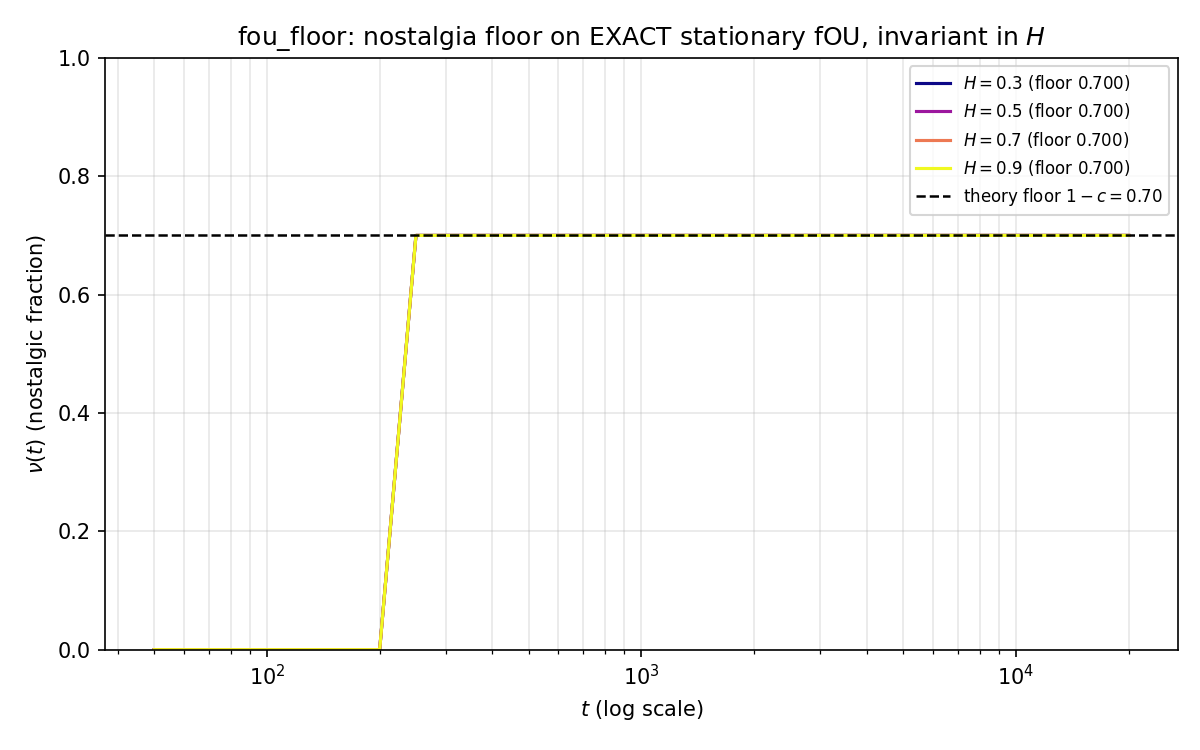
\includegraphics[width=0.82\linewidth]{figs/fig_fou_nu_vs_H.png}}

\caption{Серия \protect\texttt{fou\_floor}, инвариантность глубины пола по \(H\) (by-construction; лог-ось \(t\)). Ностальгическая доля \(\nu(t)\) равна нулю, пока буфер моложе горизонта корреляции \(\tau_E = 200\) (ни один бит ещё не старше \(\tau_E\)), затем выходит на пол \(1-c = 0{,}700\), одинаковый для всех \(H \in \{0{,}3;0{,}5;0{,}7;0{,}9\}\) --- кривые совпадают (инвариантность глубины). Пол здесь \emph{зашит} пороговой моделью (доля свежих \(= c\) через горизонт \(\hat\rho^2(\tau_E)\)): иллюстрация инвариантности на корректных fOU-путях, а не независимое измерение --- независимую оценку глубины несёт реализованный PSP-поток (рис. 2 основного текста).}

\end{figure}



\begin{figure}

\centering

\pandocbounded{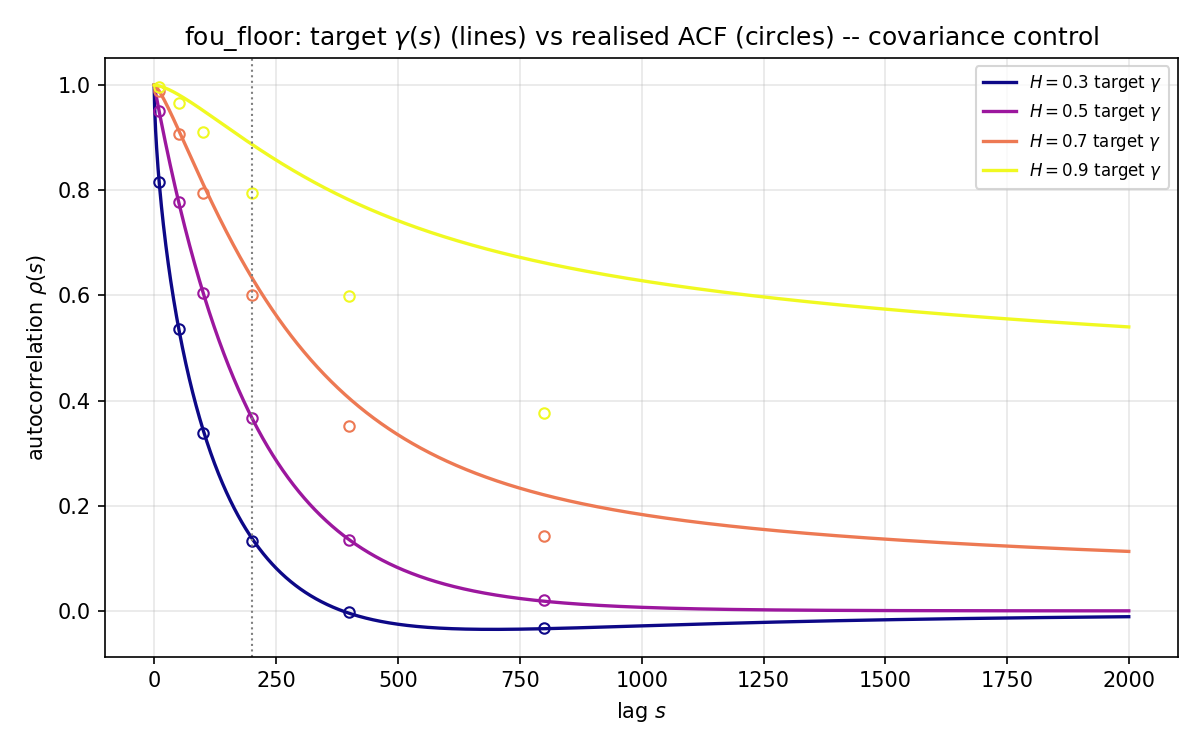
\includegraphics[width=0.82\linewidth]{figs/fig_fou_cov_control.png}}

\caption{Серия \protect\texttt{fou\_floor}, контроль ковариации. Эмпирическая лаг-корреляция реализованных путей \(\hat\rho(s)\) против целевой \(\gamma(s)\): совпадение (отн. ошибка \(<5\%\)) до лага \(\sim200\)--\(400\), где конечновыборочный оценщик ACF несмещён; на больших лагах сам оценщик ACF на долгой памяти смещён к нулю --- поэтому дальний хвост показателя читается по точной \(\gamma\), которую пути воплощают по построению, а не по выборочной ACF. Подтверждает, что генерируется подлинный стационарный fOU.}

\end{figure}



\begin{figure}

\centering

\pandocbounded{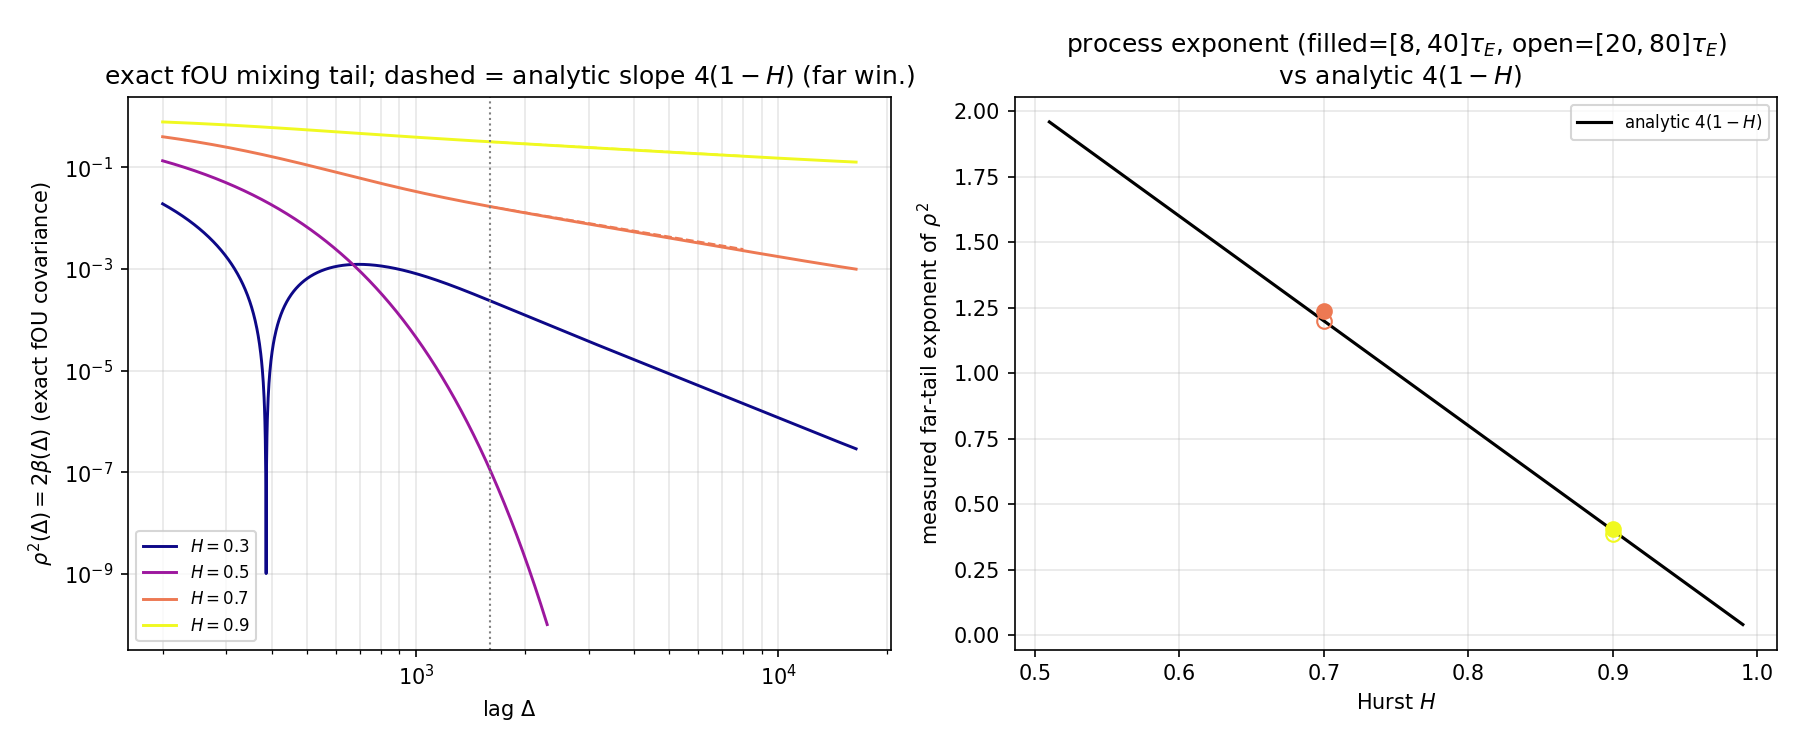
\includegraphics[width=0.82\linewidth]{figs/fig_fou_approach.png}}

\caption{Серия \protect\texttt{fou\_floor}, выход на пол и показатель скорости. Хвост \(\rho^2(\Delta) = 2\beta(\Delta)\) по точной ковариации для \(H \in \{0{,}3;0{,}5;0{,}7;0{,}9\}\); дальне-хвостовой лог-лог-наклон совпадает с аналитическим \(4(1-H)\) (внутритеоремно при \(H = 0{,}7\): \(1{,}24/1{,}20\); численно поддержанная гипотеза при \(H = 0{,}9\): \(0{,}41/0{,}39\)). При \(H = 0{,}5\) хвост экспоненциальный (OU-контроль). Показатель --- \emph{асимптотический дальне-хвостовой}: за OU-«коленом», не в наименьшем окне.}

\end{figure}



\subsection{\texorpdfstring{S4.3 \texttt{psp\_floor} (Теорема 2, экспоненциальный конец)}{S4.3 psp\_floor (Теорема 2, экспоненциальный конец)}}\label{s4.3-psp_floor-ux442ux435ux43eux440ux435ux43cux430-2-ux44dux43aux441ux43fux43eux43dux435ux43dux446ux438ux430ux43bux44cux43dux44bux439-ux43aux43eux43dux435ux446}



\textbf{Реальная траекторная симуляция} PSP-суррогата \cite{Andriishin2026b} § 6.1 (а не пересчёт \(e^{-\mu\Delta}\)): \(k = 8\), \(K = 56\); каждая координата несёт \emph{реализованный} пуассоновский поток сбросов интенсивности \(\mu \in \{10^{-3}, 3\cdot10^{-3}, 10^{-2}\}\) (пошаговая вероятность сброса \(1 - e^{-\mu}\)). \(|M| = 400\) подобрано под \(c \approx 0{,}3\) для каждого \(\mu\) (\(\tau_E = 1/\mu\)); \(T = 2\cdot10^4\), 40 реализаций, зерно \(20260528\). FIFO-память хранит снимки с меткой координаты; удержанный бит остаётся предсказательным, пока его координата \emph{фактически} не сбросилась с момента записи, и становится ностальгическим в шаг сброса. Пол и скорость декорреляции читаются из реализованного процесса. Скорость оценивается по эмпирической кривой выживания \(\hat S(\text{возраст})\) (доля удержанных битов данного возраста, ещё не увидевших сброс): фит \(\ln\hat S \sim -\text{rate}\cdot\text{возраст}\) на \([0, \min(5\tau_E,\,|M|/\dot M_{\text{refresh}})] \approx [0, 3{,}3\tau_E]\) (биты вытесняются FIFO на возрасте \(|M|/\dot M_{\text{refresh}} = \tau_E/c \approx 3{,}3\tau_E\)) в полулогарифмических координатах, с bootstrap-ДИ по реализациям; равенство скорости \(\mu\) не постулируется. \emph{Фактический выход:} установившийся эмпирический пол \(\hat\nu_{\text{floor}} = 0{,}709\text{–}0{,}713 \approx 1-c = 0{,}70\) на 10-кратном диапазоне \(\mu\) (разброс \(0{,}004\)) --- инвариантность к \(\mu\) подтверждена; поскольку процесс реализованный, установившийся пол чуть \emph{выше} \(0{,}70\) (значение пола не зашито в порог). Покадровая нижняя огибающая (колонка \texttt{liminf} в \texttt{results\_summary}) опускается до \(\approx0{,}69\) из-за конечно-выборочного шума по 40 реализациям, но \emph{медианный установившийся} уровень \(\hat\nu_{\text{floor}}\) --- выше \(1-c\); для инвариантности глубины пола релевантен установившийся уровень. Реализованная скорость декорреляции равна \(1{,}01\cdot10^{-3},\,3{,}01\cdot10^{-3},\,1{,}00\cdot10^{-2}\), и каждый bootstrap-ДИ \emph{накрывает} номинальный \(\mu = 1/\tau_E\) (S2.3) --- настоящее измерение шкалы \(1/\mu\). Расхождений с теорией нет: экспоненциальная скорость \(\mu\) подтверждена здесь, степенной показатель \(4(1-H)\) --- в \texttt{fou\_floor} (на корректном стационарном fOU, дальний хвост, § S4.2). Инвариантность установившегося пола к частоте сбросов \(\mu\) (несущее независимое свидетельство глубины C2) показана на рис. 2 основного текста.



\begin{figure}

\centering

\pandocbounded{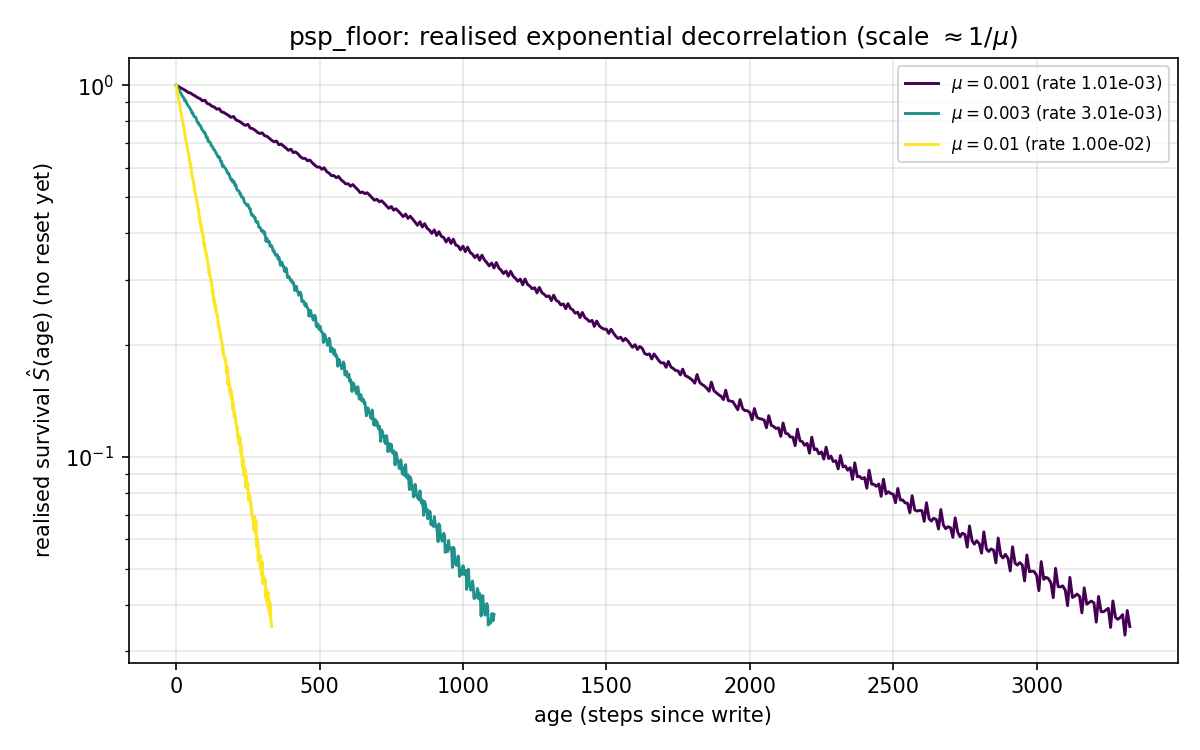
\includegraphics[width=0.82\linewidth]{figs/fig_psp_approach.png}}

\caption{Серия \protect\texttt{psp\_floor}, реализованная кривая выживания \(\hat S(\text{возраст})\) (доля удержанных битов данного возраста, ещё не увидевших сброс) в полулогарифмических координатах. Наклон даёт скорость декорреляции \(1{,}01\cdot10^{-3},\,3{,}01\cdot10^{-3},\,1{,}00\cdot10^{-2}\); каждый bootstrap-ДИ накрывает номинальный \(\mu = 1/\tau_E\) --- настоящее измерение шкалы \(1/\mu\) из реализованного процесса (равенство \(\mu\) не постулируется).}

\end{figure}



\subsection{\texorpdfstring{S4.4 \texttt{superlinear\_memory} (Теорема 3)}{S4.4 superlinear\_memory (Теорема 3)}}\label{s4.4-superlinear_memory-ux442ux435ux43eux440ux435ux43cux430-3}



Память \(|M_{\le t}| = M_0 t^\alpha\), \(\alpha \in \{1, 1{,}5, 2, 3\}\), плюс экспоненциальная \(|M_{\le t}| = M_0 e^{\kappa t}\) с \(\kappa\tau_E \in \{0{,}1, 0{,}5, 1\}\). OU-дрейф фоновой среды, \(\tau_E = 200\), FIFO-refresh, зерно \(20260529\). Измеряется \(\nu(t)\), доля свежих битов \(\phi(t)\) (S3.1), и для экспоненциального случая --- кумулятивная \(E_{\text{grow}}(t)\) и \(\eta_L(t)\). \emph{Фактический выход:} для всех полиномиальных \(\alpha\) --- \(\phi(t) \sim t^{-\gamma}\) с \(\gamma \in \{1{,}000;\,0{,}991;\,0{,}982;\,0{,}964\}\) (разброс \(0{,}036\), \(\gamma \approx 1\) независимо от \(\alpha\)), префактор \(\phi\cdot t \to \alpha\tau_E\) (\(200,\,298,\,394,\,581\) против \(200,\,300,\,400,\,600\)), \(\nu(t) \to 1\) (S3.2--S3.3) --- подтверждение отсутствия полиномиального \(\alpha_c\); малое отклонение \(\gamma\) от \(1\) при больших \(\alpha\) --- конечно-оконный subleading-артефакт, ведущий показатель тождественно \(1\). \emph{Диагностика сходимости окна} (\texttt{gamma\_window\_convergence} в \texttt{results\_summary}; детерминированная табуляция точного \(\phi = 1-((t-\tau_E)/t)^\alpha\), не Монте-Карло): при скольжении окна фита (декада \([w, 10w]\)) вправо показатель \(\gamma\) монотонно растёт к \(1\) для \emph{каждого} \(\alpha\) --- при подъёме окна на порядок (\(w = 2\cdot10^4\)) \(\gamma \to \{1{,}000;\,0{,}999;\,0{,}998;\,0{,}996\}\), при \(\times1000\) (\(w = 2\cdot10^6\)) \(\gamma \to \{1{,}000;\,1{,}000;\,1{,}000;\,1{,}000\}\) при \(\alpha \in \{1;\,1{,}5;\,2;\,3\}\); локальный лог-лог-наклон \(\phi\) садится к \(-1\) (\(-0{,}897 \to -0{,}990 \to -0{,}999 \to \dots \to -1{,}000\) при \(t = 2\cdot10^3 \dots 2\cdot10^9\)). Тем самым дрейф \(\gamma\) вниз на baseline-окне --- subleading-кривизна конечного окна, а не зависимость ведущего показателя от \(\alpha\); ведущий показатель тождественно \(1\), и полиномиального \(\alpha_c\) нет. Для экспоненциального роста --- \(\phi_\infty = 1-e^{-\kappa\tau_E} \in \{0{,}095;\,0{,}394;\,0{,}632\} > 0\), \(\nu(t) < 1\), но \(E_{\text{grow}}(t) \propto e^{\kappa t}\) расходится (отношение до \(9{,}8\cdot10^{42}\) за прогон) и \(\eta_L(t) \to 0\) через знаменатель (S3.5--S3.6). Насыщение \(\phi(t)\to0\) при полиномиальном росте (отсутствие \(\alpha_c\)) показано на рис. 3 основного текста.



\begin{figure}

\centering

\pandocbounded{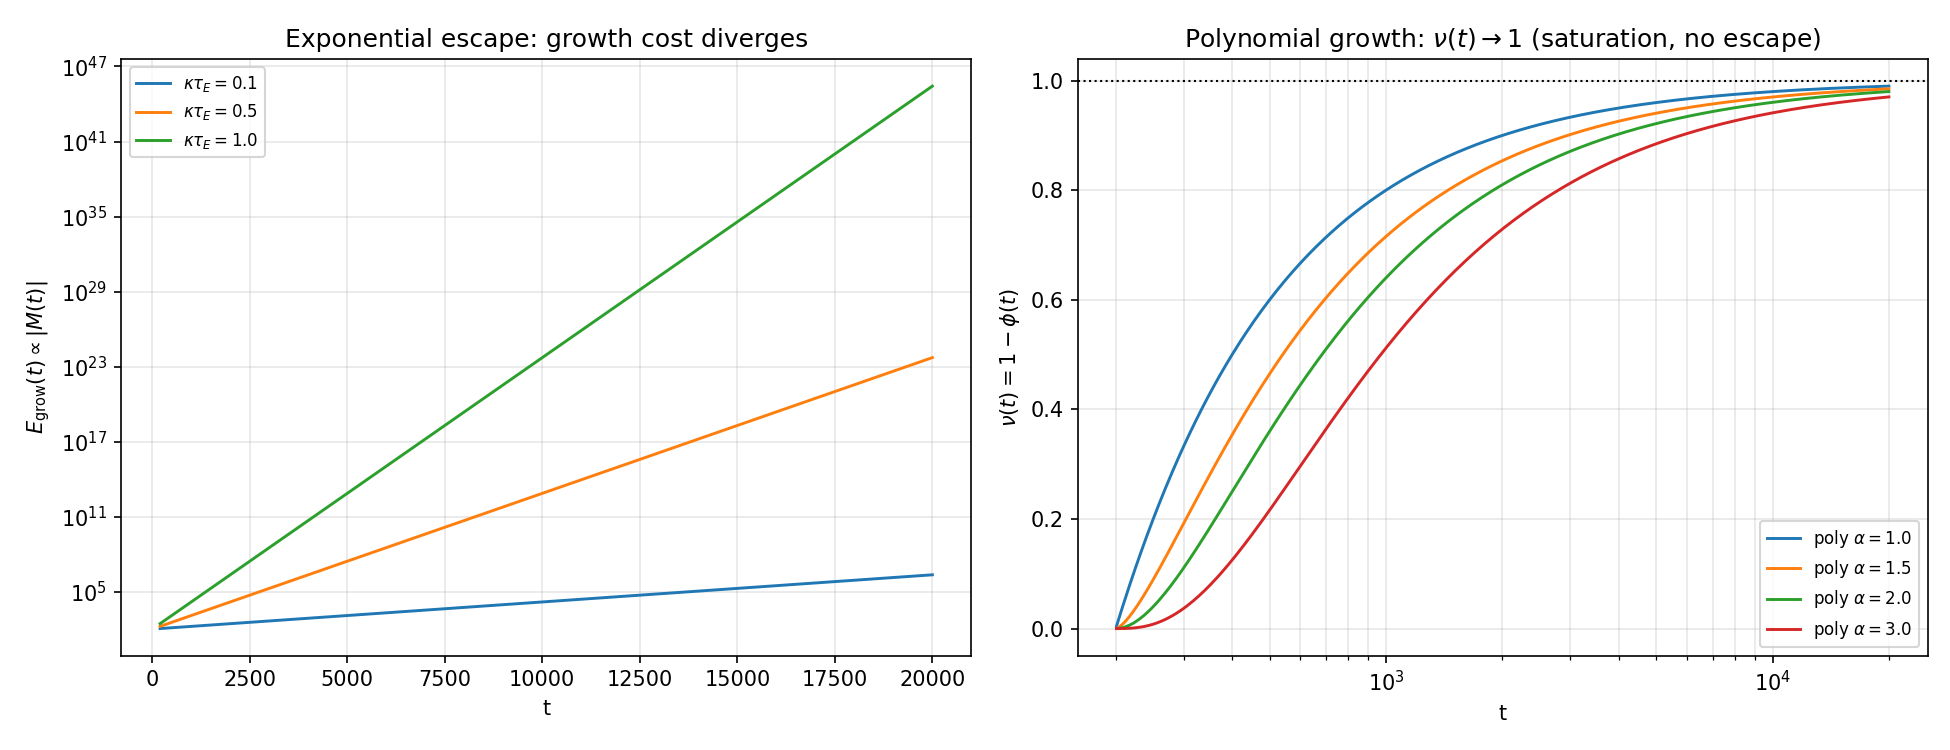
\includegraphics[width=0.82\linewidth]{figs/fig_superlinear_escape.png}}

\caption{Серия \protect\texttt{superlinear\_memory}, экспоненциальный побег и его цена. При \(|M_{\le t}| = M_0 e^{\kappa t}\) доля свежих выходит на ненулевой предел \(\varphi_\infty = 1-e^{-\kappa\tau_E} \in \{0{,}095;0{,}394;0{,}632\}\) (побег: \(\nu < 1\)), но кумулятивная стоимость расширения ёмкости \(E_{\text{grow}}(t) \propto e^{\kappa t}\) расходится (отношение до \(9{,}8\cdot10^{42}\)), и эффективность \(\eta_L(t) \to 0\) через знаменатель. Побег формально удерживает ностальгию ниже \(1\), но термодинамически разорителен.}

\end{figure}



\subsection{S4.5 Общие конвенции и ограничения}\label{s4.5-ux43eux431ux449ux438ux435-ux43aux43eux43dux432ux435ux43dux446ux438ux438-ux438-ux43eux433ux440ux430ux43dux438ux447ux435ux43dux438ux44f}



Во всех сериях истинное \(\theta(t)\) известно по построению, поэтому \(\nu^{\text{theor}} = \nu^{\text{op}}\) \cite{Andriishin2026b} § 6; используется \(\nu(t)\) без индекса. \emph{Оговорка об оценщике.} В численных сериях \#3 (\texttt{fou\_floor}, \texttt{psp\_floor}) ностальгия \(\nu(t)\) читается не KSG-оценщиком взаимной информации, а из \emph{пороговой DPI-модели горизонта}: бит возраста \(\Delta\) считается полезным, если его предсказательная ценность по реализованной автокорреляции \(\hat\rho^2(\Delta)\) (survival на известном \(\theta(t)\)) превышает DPI-порог \(\rho^2(\tau_E)\), иначе --- ностальгическим. Поскольку \(\theta(t)\) известно по построению, обусловливание на латент реализуется \emph{фиксацией} истинного \(\theta\), и условная \(I_{\text{pred}} = I(X_t;X_{t+\tau}\mid\theta(t))\) измеряется напрямую --- отсюда \(\nu^{\text{theor}} = \nu^{\text{op}}\) by construction; отдельный CMI-оценщик не требуется. Упоминание KSG \cite{Andriishin2026b} § S6 наследуется от сопровождающей работы \#2 и к численным сериям \#3 \emph{не применяется} (там \(\theta\) известно по построению). Симуляции иллюстрируют, но не доказывают теоремы (§ S1--S3 несут доказательства); не выходят за пределы абстрактных марковских цепей; не покрывают не-перемешивающийся (heavy-tailed) класс вне области Теоремы 2. Полная реализация, зёрна, псевдокод и регенерация рисунков --- в \texttt{simulations/\{ou\_adiab,fou\_floor,psp\_floor,superlinear\_memory\}/README.md} репозитория-зеркала \texttt{andriishin/landauer-undertow-oa}.



\section*{References}
\bibliographystyle{iopart-num}
\bibliography{refs}

\end{document}
